\chapter{実験と検証}
提案手法によって\ref{classify-model}節で構築した分類モデルと\ref{generate-model}節で構築した生成モデルの評価を行う.また\ref{visualize}節のように生成モデルから得られる2次元ジャンルマップ空間に対し検証を行う.


\section{分類モデルの評価}
\subsection{学習毎の損失と精度のグラフ}
\ref{classify-model}節の学習毎のCNNにおいて,1データ当たり3秒間の学習データとテストデータの組み合わせを変えた実験を行う.合計10通りの組み合わせを行ったとき,それぞれの学習毎のモデルにおける分類時の損失と精度をグラフにプロットしたものを\figref{fig:CNNmel0}~\figref{fig:CNNmel9}に示す.横軸は学習回数(epoch),縦軸はその時の損失と精度を表している.
\begin{figure}[htbp]
	\begin{center}
		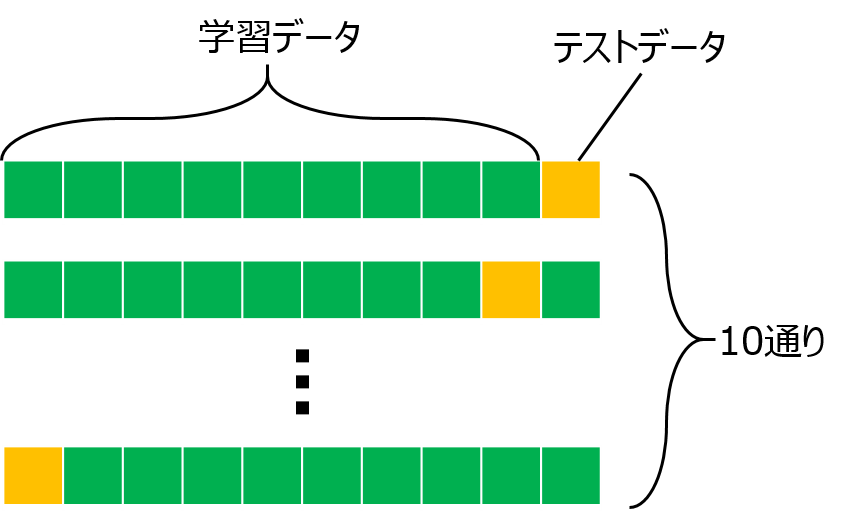
\includegraphics[scale=0.7]{./images/dataset/crossval.png}
		\caption{10分割交差検証}
		\label{fig:crossvalidation}
	\end{center}
\end{figure}

\begin{figure}
	\begin{center}
		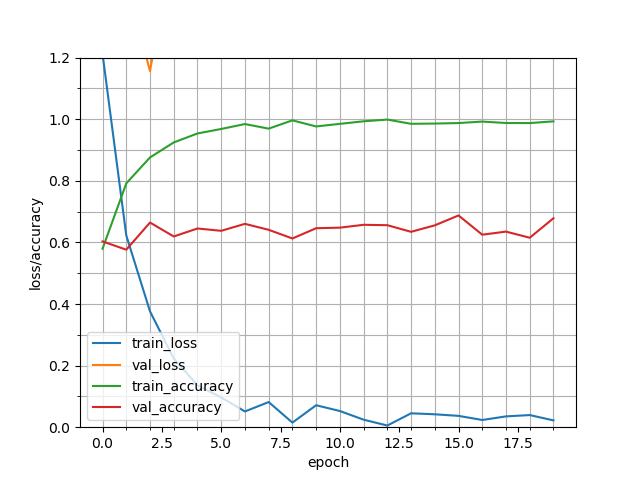
\includegraphics[scale=0.8]{./images/classify-model/loss_acuuracy_CNN_mel_0.png}
		\caption{損失と精度パターン0}
		\label{fig:CNNmel0}
		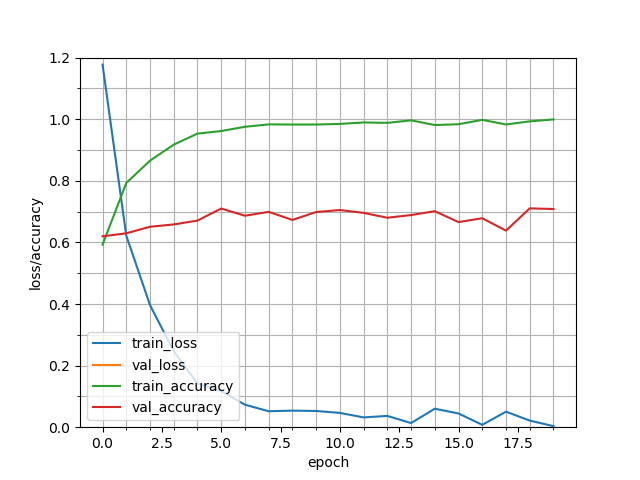
\includegraphics[scale=0.8]{./images/classify-model/loss_acuuracy_CNN_mel_1.png}
		\caption{損失と精度パターン1}
		\label{fig:CNNmel1}
	\end{center}
\end{figure}
\begin{figure}
	\begin{center}
		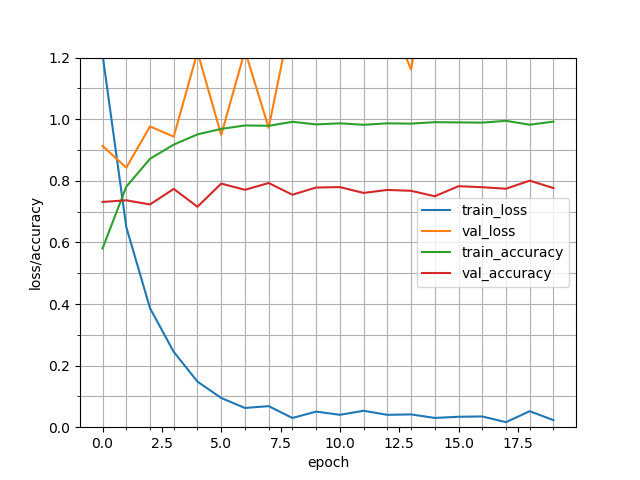
\includegraphics[scale=0.8]{./images/classify-model/loss_acuuracy_CNN_mel_2.png}
		\caption{損失と精度パターン2}
		\label{fig:CNNmel2}
		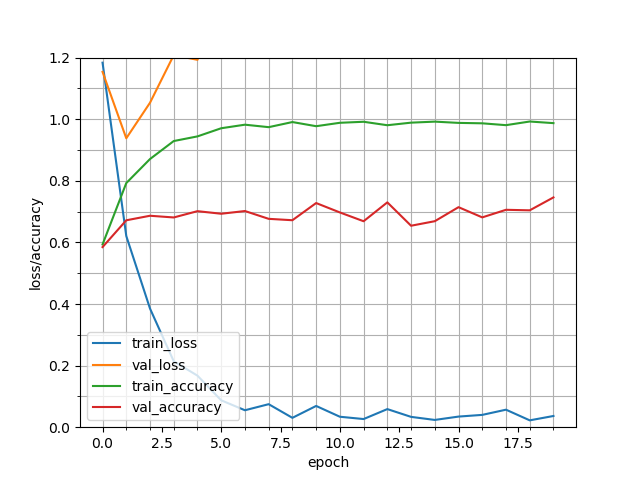
\includegraphics[scale=0.8]{./images/classify-model/loss_acuuracy_CNN_mel_3.png}
		\caption{損失と精度パターン3}
		\label{fig:CNNmel3}
	\end{center}
\end{figure}
\begin{figure}
	\begin{center}
		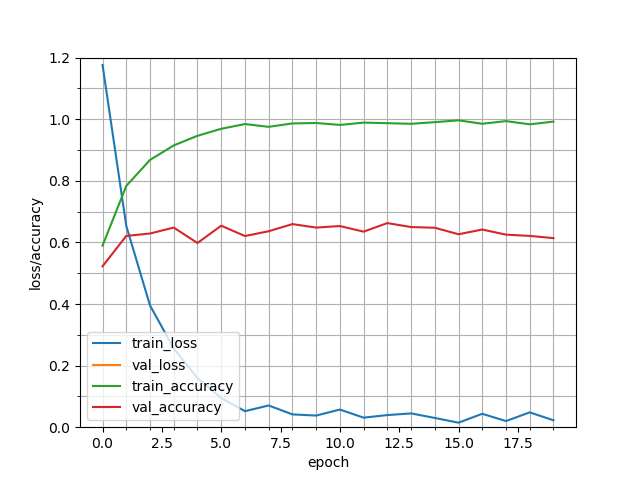
\includegraphics[scale=0.8]{./images/classify-model/loss_acuuracy_CNN_mel_4.png}
		\caption{損失と精度パターン4}
		\label{fig:CNNmel4}
		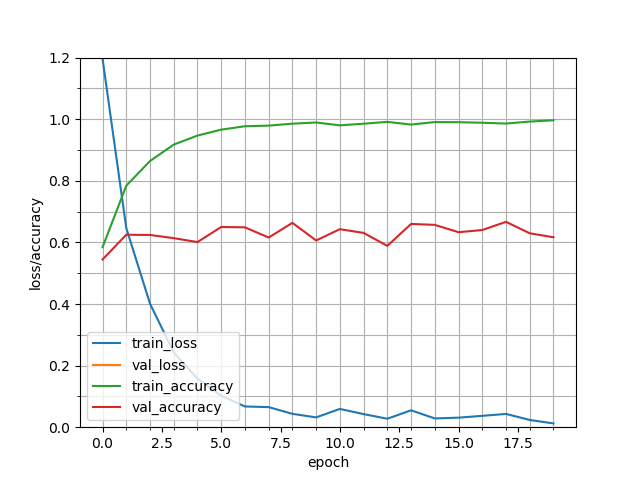
\includegraphics[scale=0.8]{./images/classify-model/loss_acuuracy_CNN_mel_5.png}
		\caption{損失と精度パターン5}
		\label{fig:CNNmel5}
	\end{center}
\end{figure}
\begin{figure}
	\begin{center}
		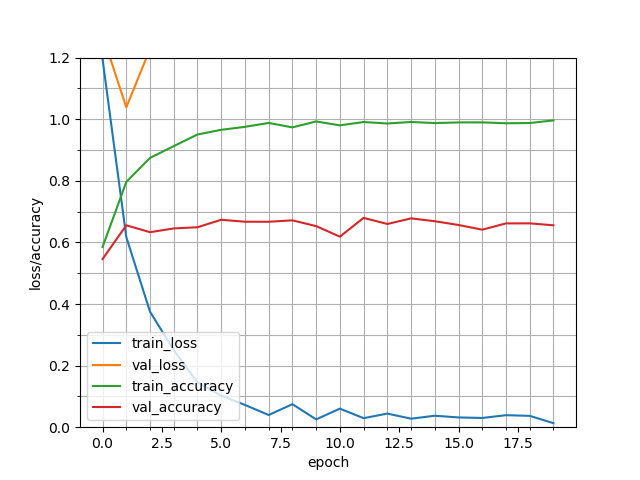
\includegraphics[scale=0.8]{./images/classify-model/loss_acuuracy_CNN_mel_6.png}
		\caption{損失と精度パターン6}
		\label{fig:CNNmel6}
		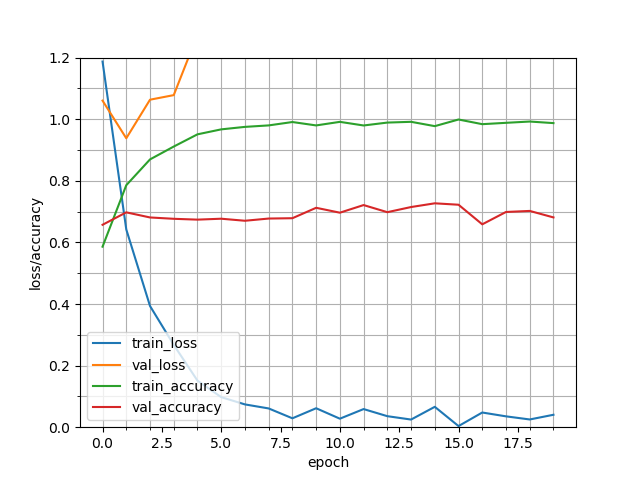
\includegraphics[scale=0.8]{./images/classify-model/loss_acuuracy_CNN_mel_7.png}
		\caption{損失と精度パターン7}
		\label{fig:CNNmel7}
	\end{center}
\end{figure}
\begin{figure}
	\begin{center}
		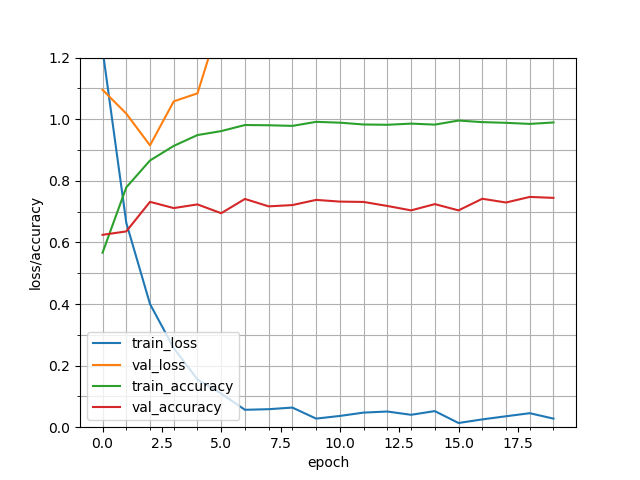
\includegraphics[scale=0.8]{./images/classify-model/loss_acuuracy_CNN_mel_8.png}
		\caption{損失と精度パターン8}
		\label{fig:CNNmel8}
		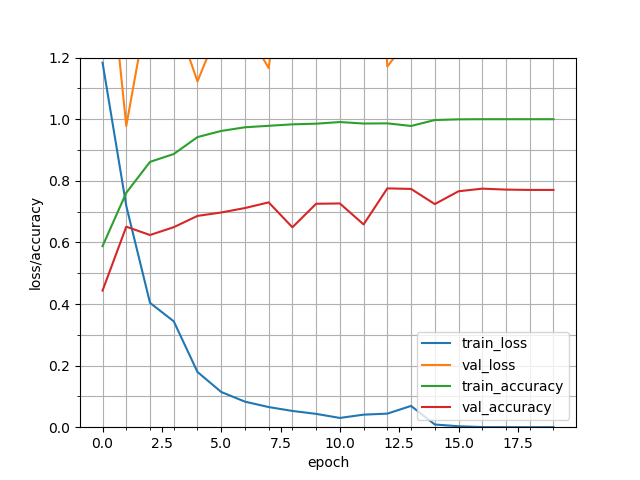
\includegraphics[scale=0.8]{./images/classify-model/loss_acuuracy_CNN_mel_9.png}
		\caption{損失と精度パターン9}
		\label{fig:CNNmel9}
	\end{center}
\end{figure}

\newpage
\figref{fig:CNNmel0}~\figref{fig:CNNmel9}より,学習データの組み合わせによって,テストデータに対する分類精度が大きく影響しているということが読み取れる.特に\figref{fig:CNNmel2}より,パターン2のデータセットを用いたときにおけるテストデータの精度が一番高いため,データセット2を用いた学習済みCNNはより最適解に近い学習を行ったと言える.よって学習済みCNNから特徴を分析する際には,学習データセットをパターン2に設定したモデルを使用することで,より信頼性のあるジャンル境界線を可視化できると考えられる.

\subsection{1曲分の分類精度}
\figref{fig:classify30s}のように1曲30秒間のテストデータを3秒ごとに分類し,多数決をとったものを1曲分のジャンル分類結果として評価した場合の精度を示す.10通りのモデルセットにおけるテストデータを\figref{fig:classify30s}のように分類していき,精度を算出した際の混同行列を\figref{fig:CNN0}~\figref{fig:CNN9}に示す.また10パターンのモデル精度を平均した時の混同行列を\figref{fig:crossval}に示す.
\begin{figure}[htbp]
	\begin{center}
		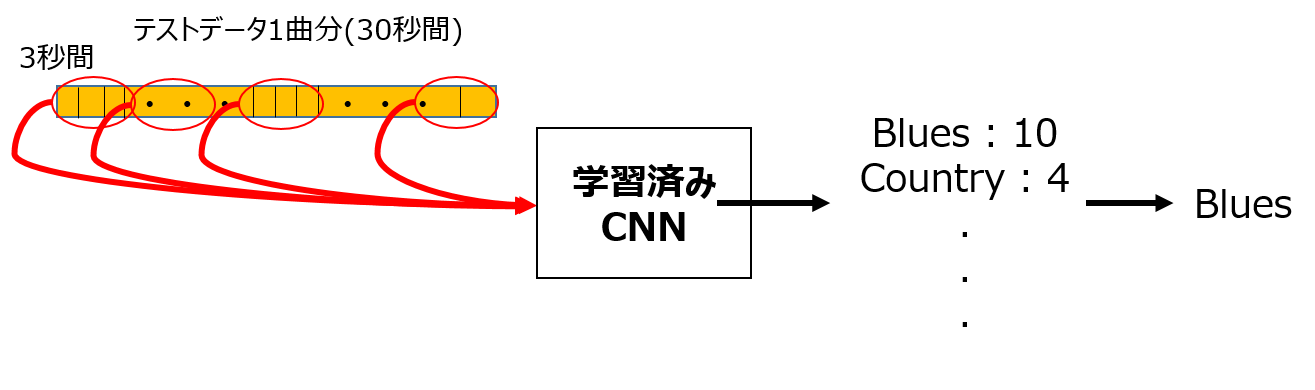
\includegraphics[scale=0.7]{./images/classify-model/classify30s.png}
		\caption{1曲分の分類精度}
		\label{fig:classify30s}
	\end{center}
\end{figure}
\newpage
\begin{figure}[htbp]
	\begin{center}
		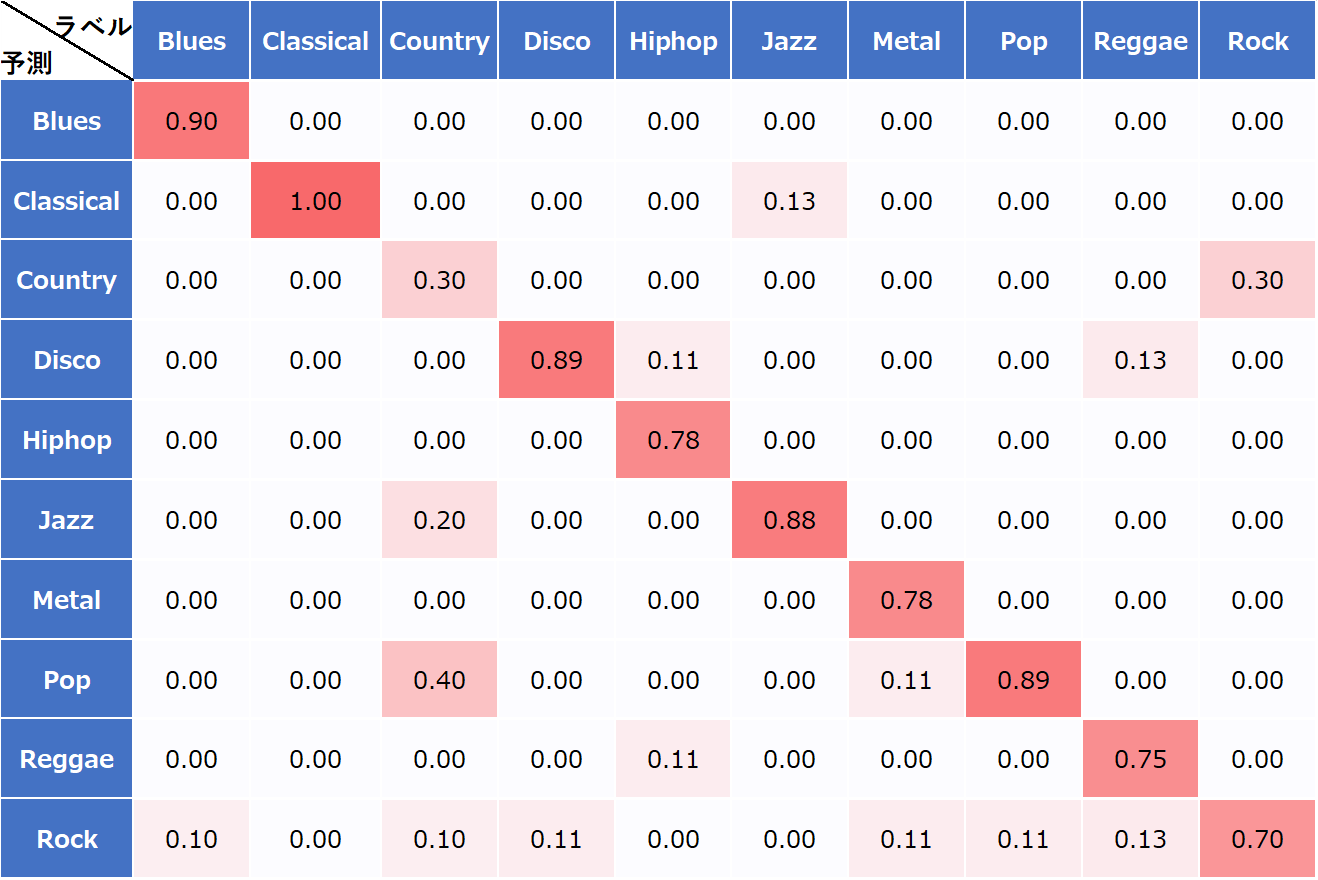
\includegraphics[scale=0.48]{./images/classify-model/mel0_matrix.png}
		\caption{ジャンル毎の分類精度:パターン0}
		\label{fig:CNN0}
		\vspace{50pt}
		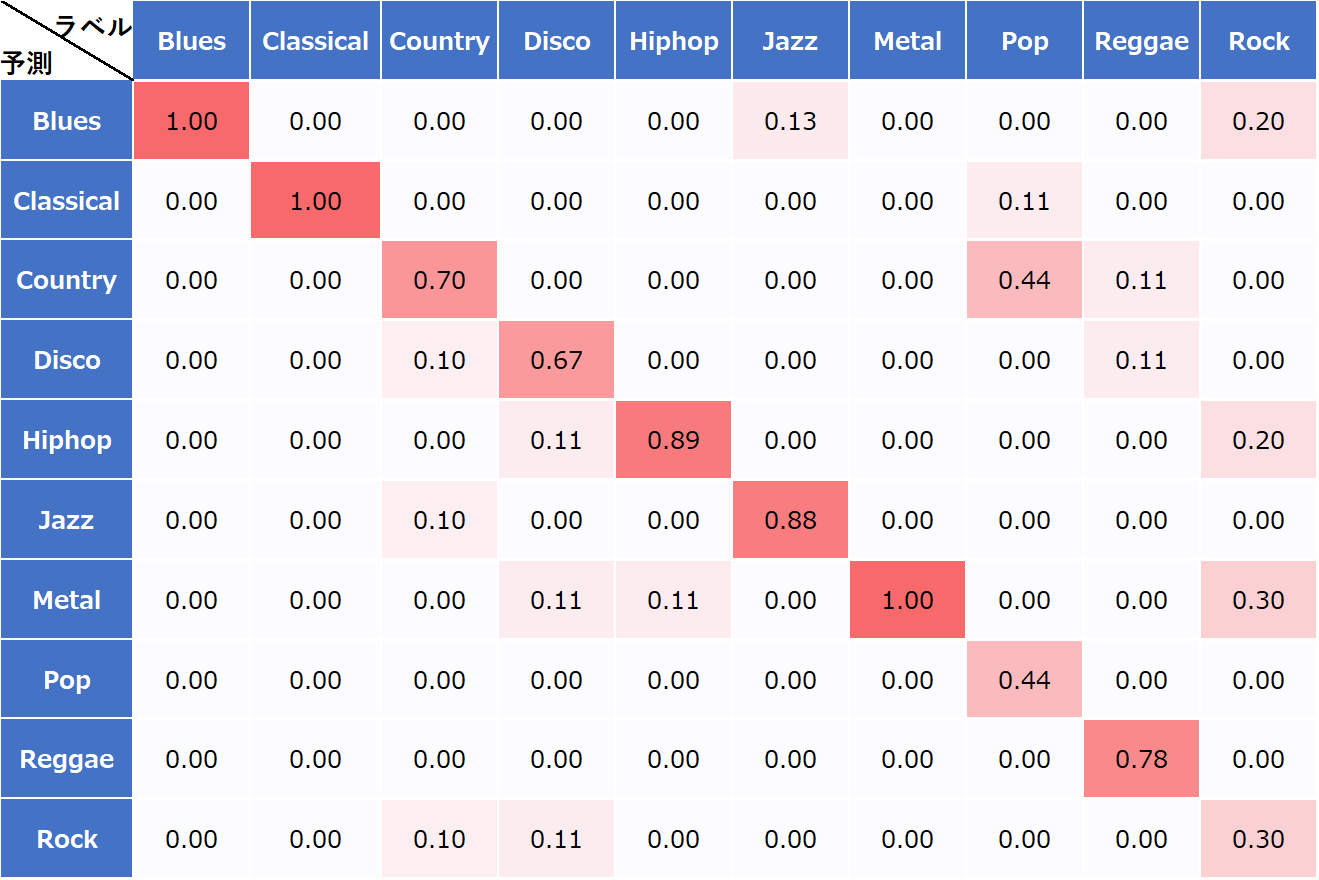
\includegraphics[scale=0.5]{./images/classify-model/mel1_matrix.png}
		\caption{ジャンル毎の分類精度:パターン1}
		\label{fig:CNN1}
	\end{center}
\end{figure}
\newpage
\begin{figure}[htbp]
	\begin{center}
		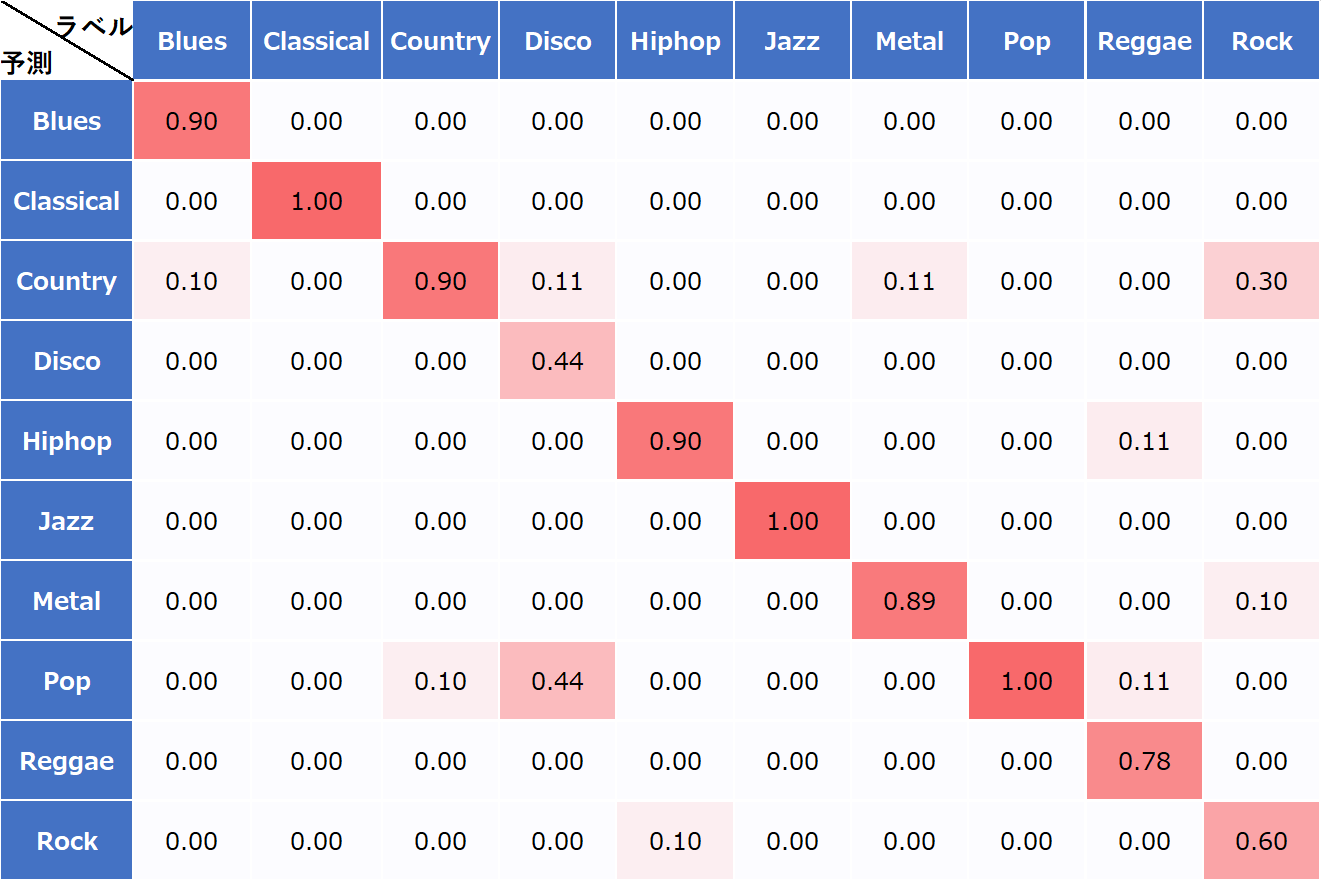
\includegraphics[scale=0.5]{./images/classify-model/mel2_matrix.png}
		\caption{ジャンル毎の分類精度:パターン2}
		\label{fig:CNN2}
		\vspace{50pt}
		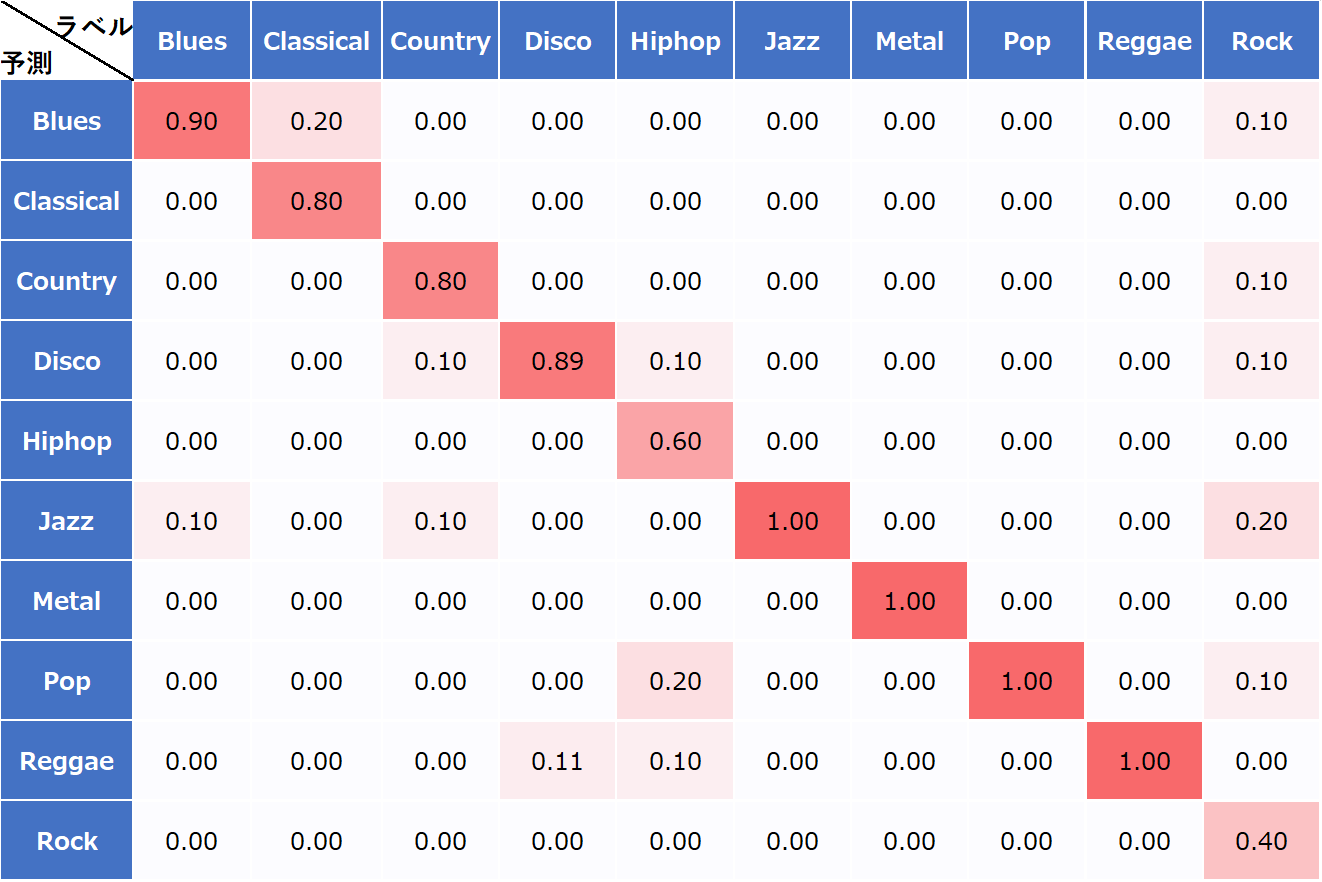
\includegraphics[scale=0.5]{./images/classify-model/mel3_matrix.png}
		\caption{ジャンル毎の分類精度:パターン3}
		\label{fig:CNN3}
	\end{center}
\end{figure}
\newpage
\begin{figure}[htbp]
	\begin{center}
		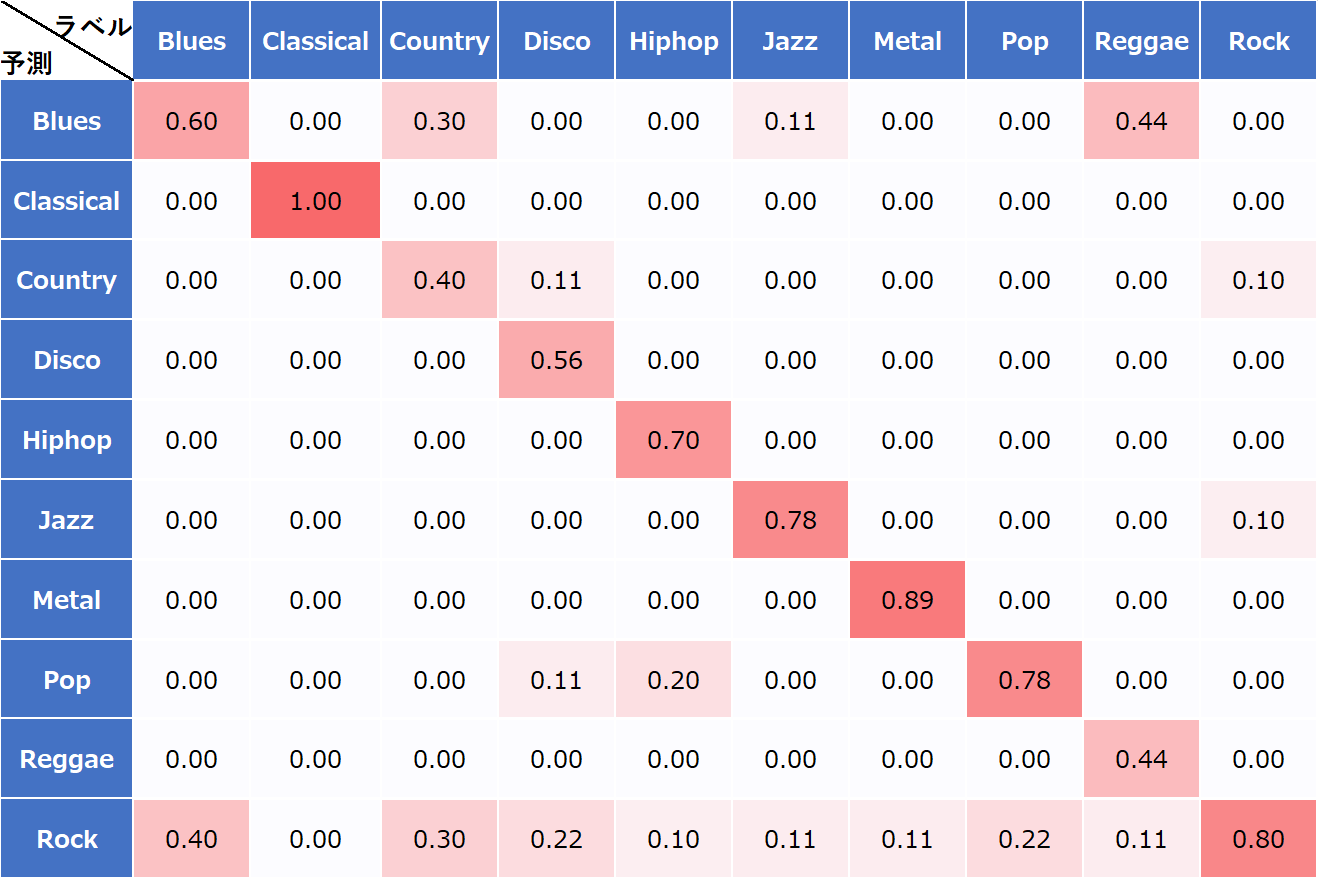
\includegraphics[scale=0.5]{./images/classify-model/mel4_matrix.png}
		\caption{ジャンル毎の分類精度:パターン4}
		\label{fig:CNN4}
		\vspace{50pt}
		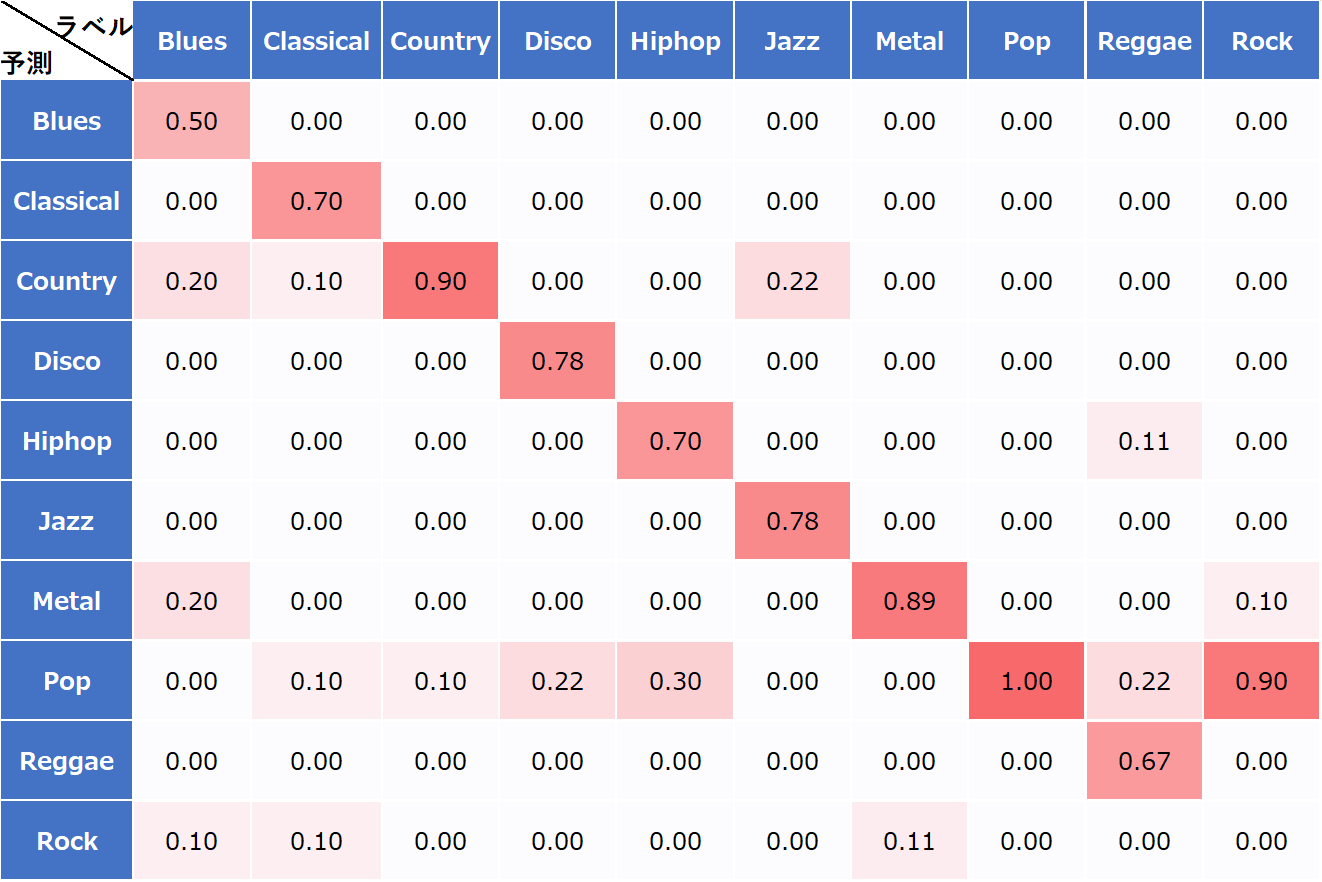
\includegraphics[scale=0.5]{./images/classify-model/mel5_matrix.png}
		\caption{ジャンル毎の分類精度:パターン5}
		\label{fig:CNN5}
	\end{center}
\end{figure}
\newpage
\begin{figure}[htbp]
	\begin{center}
		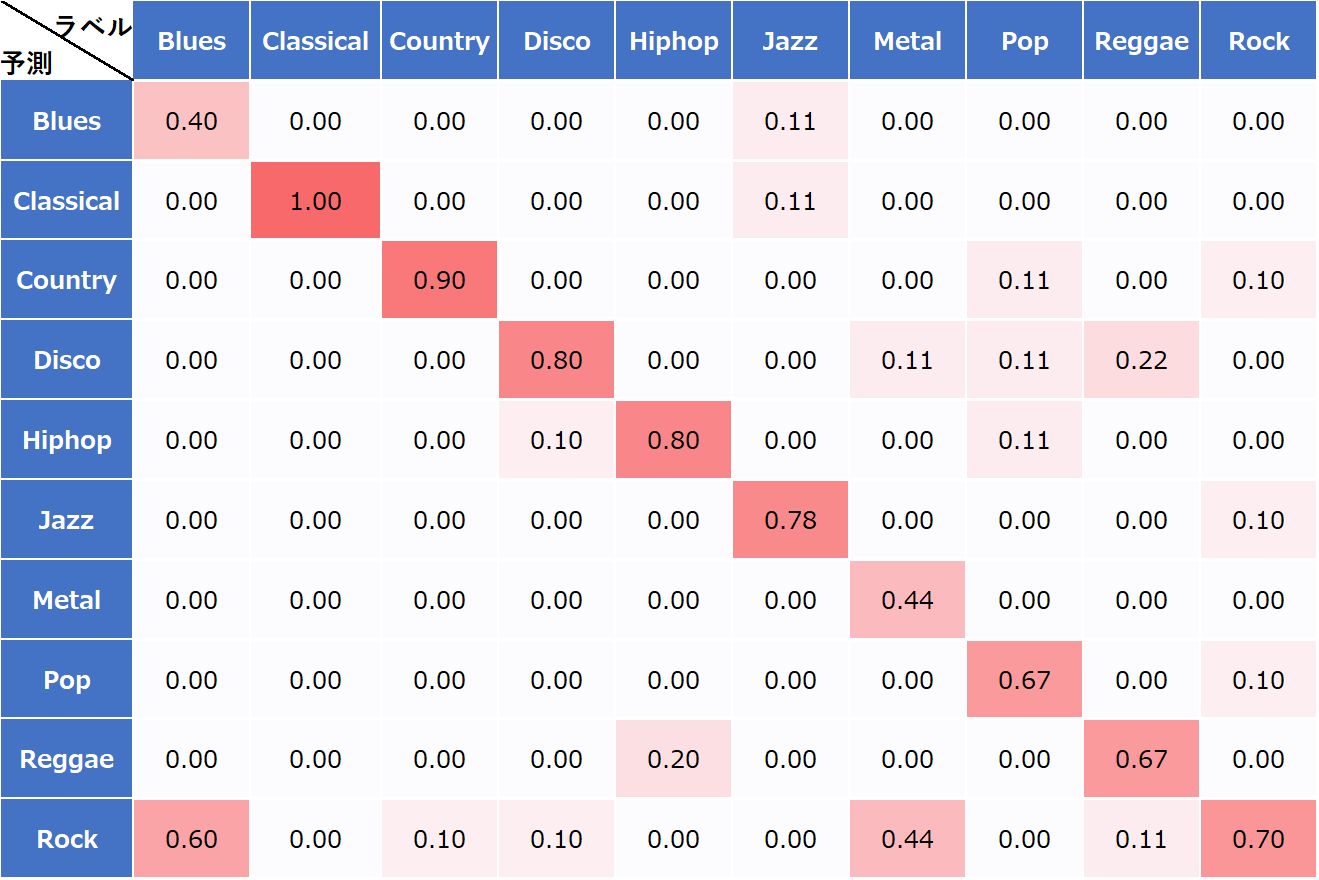
\includegraphics[scale=0.5]{./images/classify-model/mel6_matrix.png}
		\caption{ジャンル毎の分類精度:パターン6}
		\label{fig:CNN6}
		\vspace{50pt}
		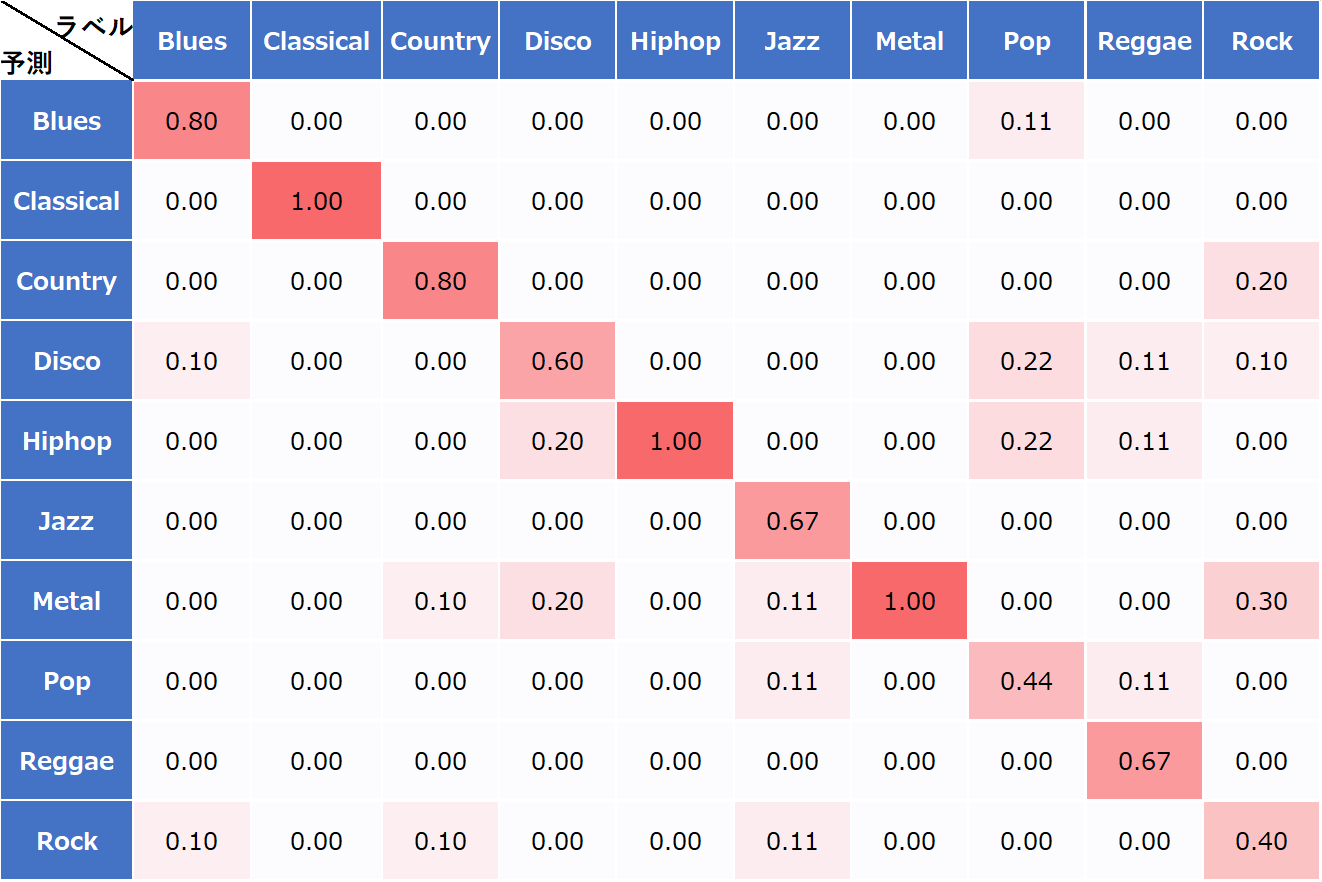
\includegraphics[scale=0.5]{./images/classify-model/mel7_matrix.png}
		\caption{ジャンル毎の分類精度:パターン7}
		\label{fig:CNN7}
	\end{center}
\end{figure}
\newpage
\begin{figure}[htbp]
	\begin{center}
		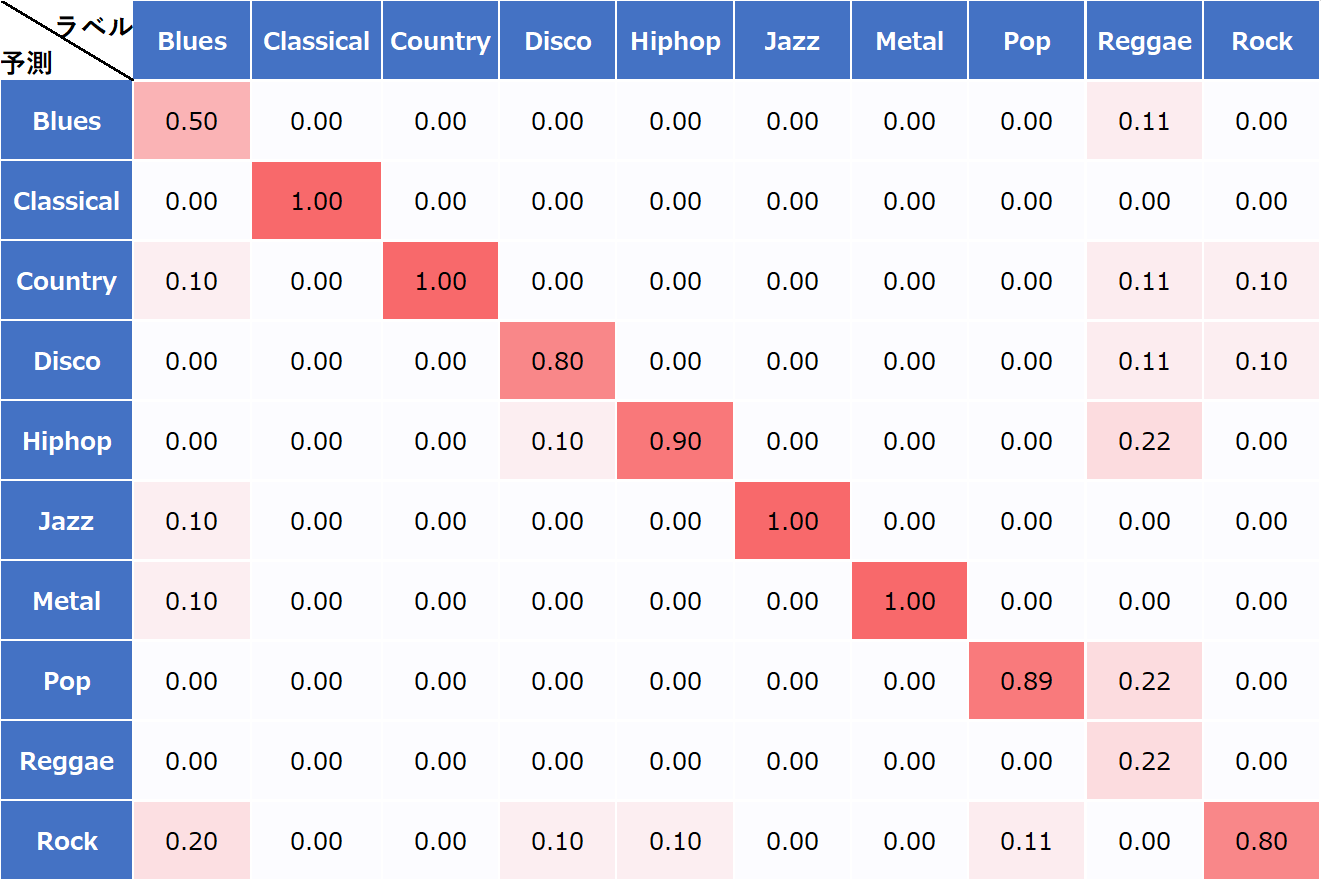
\includegraphics[scale=0.5]{./images/classify-model/mel8_matrix.png}
		\caption{ジャンル毎の分類精度:パターン8}
		\label{fig:CNN8}
		\vspace{50pt}
		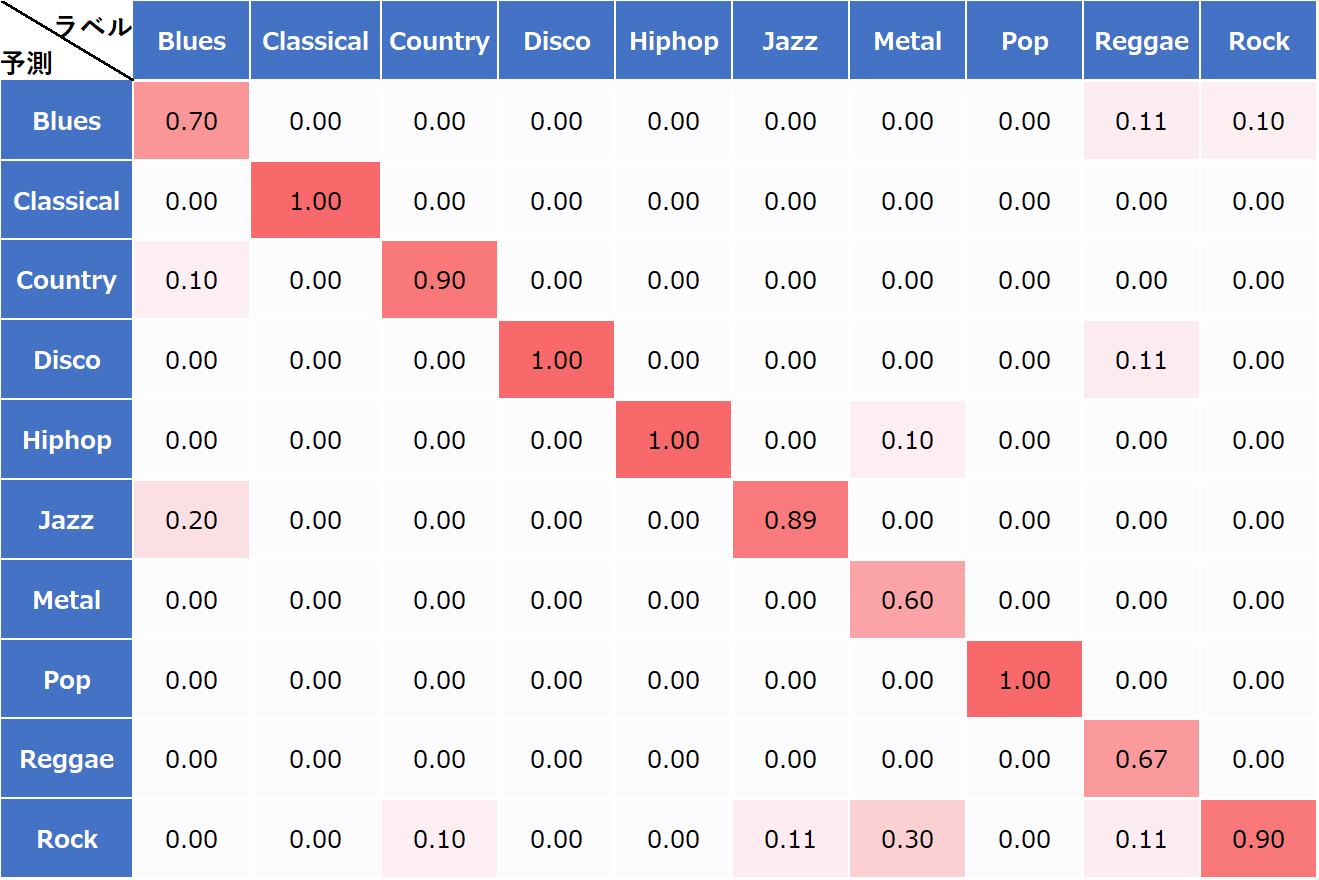
\includegraphics[scale=0.5]{./images/classify-model/mel9_matrix.png}
		\caption{ジャンル毎の分類精度:パターン9}
		\label{fig:CNN9}
	\end{center}
\end{figure}
\clearpage
\begin{figure}[htbp]
	\begin{center}
		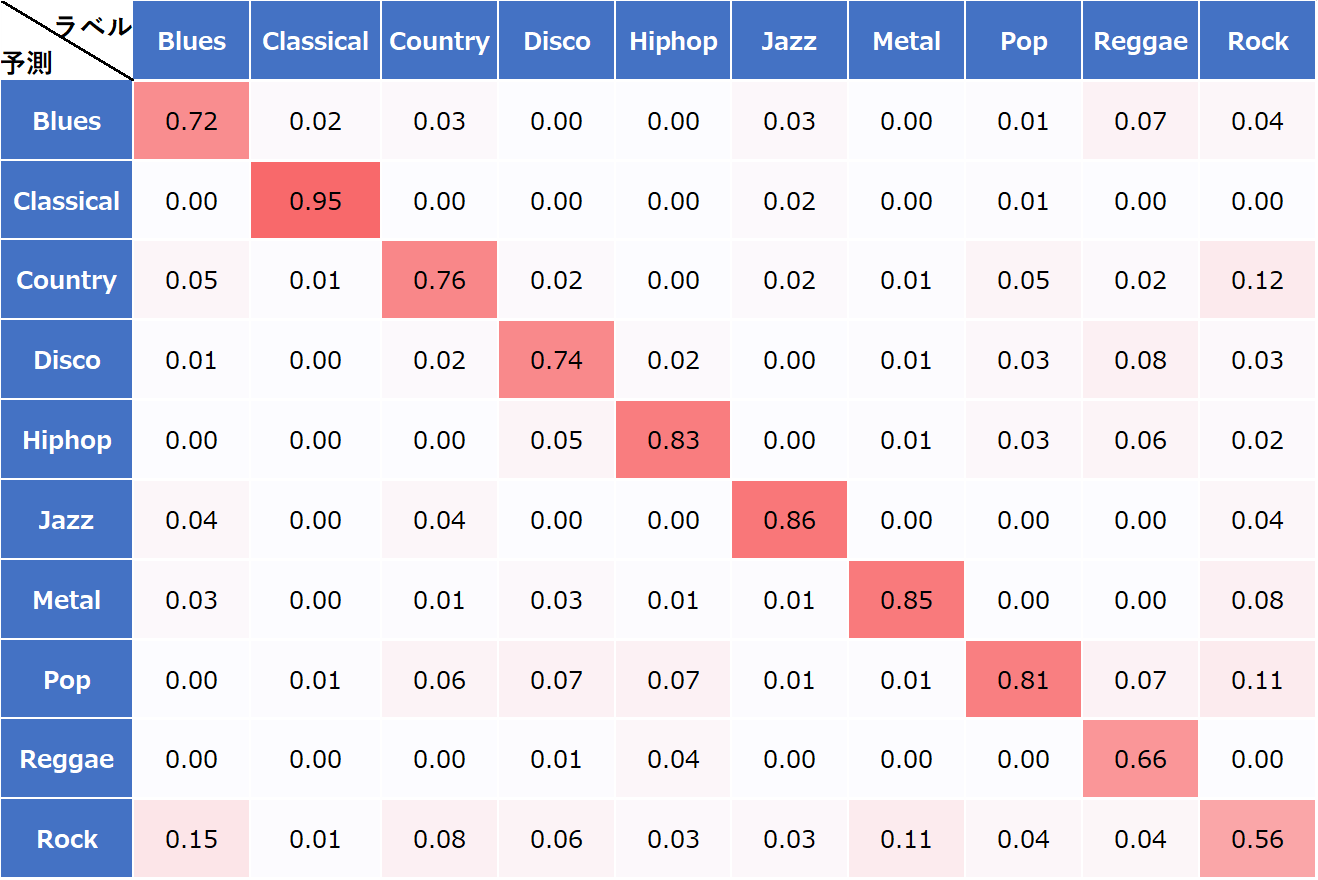
\includegraphics[scale=0.5]{./images/classify-model/crossval.png}
		\caption{平均の分類精度}
		\label{fig:crossval}
	\end{center}
\end{figure}

\figref{fig:crossval}における提案手法によるモデルの分類精度と,\figref{fig:mingwen-table}におけるMingewnらによるモデルの分類精度を比較すると,極端に低かったCountryとRockの分類精度が向上していることがわかる.また,全体的な分類精度も77.4\%となり向上した.\figref{fig:CNN0}~\figref{fig:CNN9}から,誤分類するジャンルがモデルによって変化するが,特にRockのジャンルが全体のジャンルにわたって誤分類されやすいということが分かる.すなわちRockというジャンルは他のジャンルに共通する特徴を持ちやすいということが考えられる.



\clearpage
\section{生成器モデルの評価}
\subsection{学習毎の損失}
\ref{generate-model}節において,学習毎のDiscriminatorが出力するwasserstein距離と,相互情報量を推定し最大化するNNの損失(mutual\_loss)を学習事にプロットしたものを\figref{fig:wasserstein-loss}に示す.横軸は学習回数(epoch),縦軸はその時のmutual\_lossまたはwasserstein距離を表している.

\begin{figure}[htbp]
	\begin{center}
		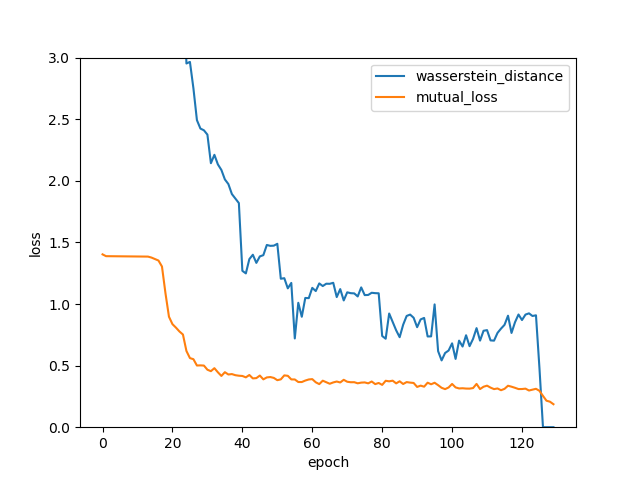
\includegraphics[scale=0.55]{./images/generate-model/lossmutual_gan_2.png}
		\caption{学習毎のwasserstein距離とNNの損失}
		\label{fig:wasserstein-loss}
	\end{center}
\end{figure}

\figref{fig:wasserstein-loss}より,Discriminatorが出力するwasserstein距離が下がっていくことが読み取れる.wasserstein距離は生成データとオリジナルデータの分布間距離を示しているため,生成データがオリジナルのスペクトログラムに近づいているということがわかる.しかし,epochが125を超えたあたりからwasserstein距離が0となり勾配が消失し,学習が失敗していることが読み取れる.そのため,wasserstein距離の学習が収束傾向であり,学習が失敗する寸前のepochが120回目のモデルで学習を止めることが最善であると考えられる.
一方mutual\_lossは\eref{eq:deepinfomax}を最小値問題としたときの目的関数の値を示している.mutual\_lossが減少していることから,Generatorの入力ランダムノイズ$z$と,$z$から得られた生成データYをCNNに入力した時に得られる特徴マップ$m$との間で相互情報量が推定され,さらに最大化されているということがわかる.よって入力ランダムノイズ$z$とCNNのジャンル出力との間に従属関係があると言える.

\clearpage
\subsection{生成されるスペクトログラム}
学習済Generatorが出力するスペクトログラムとそれらをCNNで分類した結果の一例を\figref{fig:generate-blues}~\figref{fig:generate-rock}に示す.
\begin{figure}[htbp]
	\begin{center}
		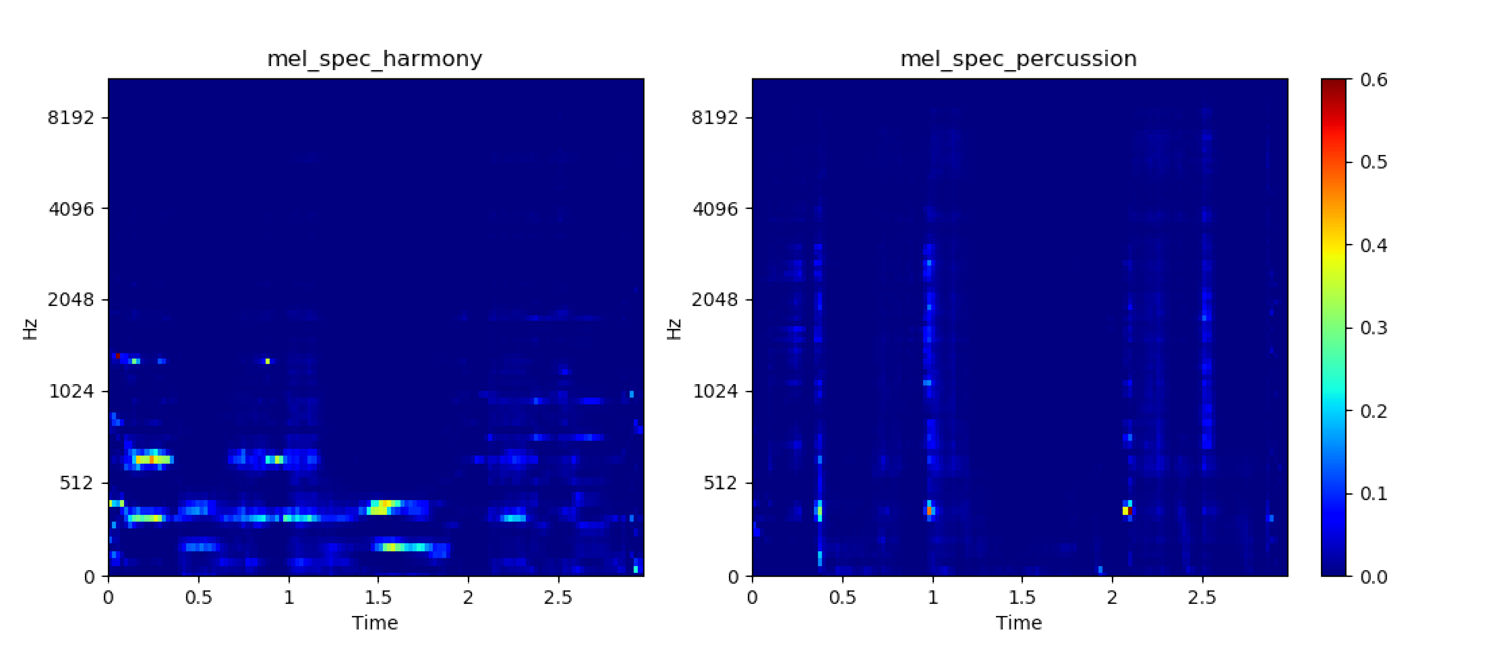
\includegraphics[scale=0.58]{./images/generate-model/gen-blues.png}
		\caption{Bluesと分類した生成スペクトログラム}
		\label{fig:generate-blues}
	\end{center}
\end{figure}
\begin{figure}[htbp]
	\begin{center}
		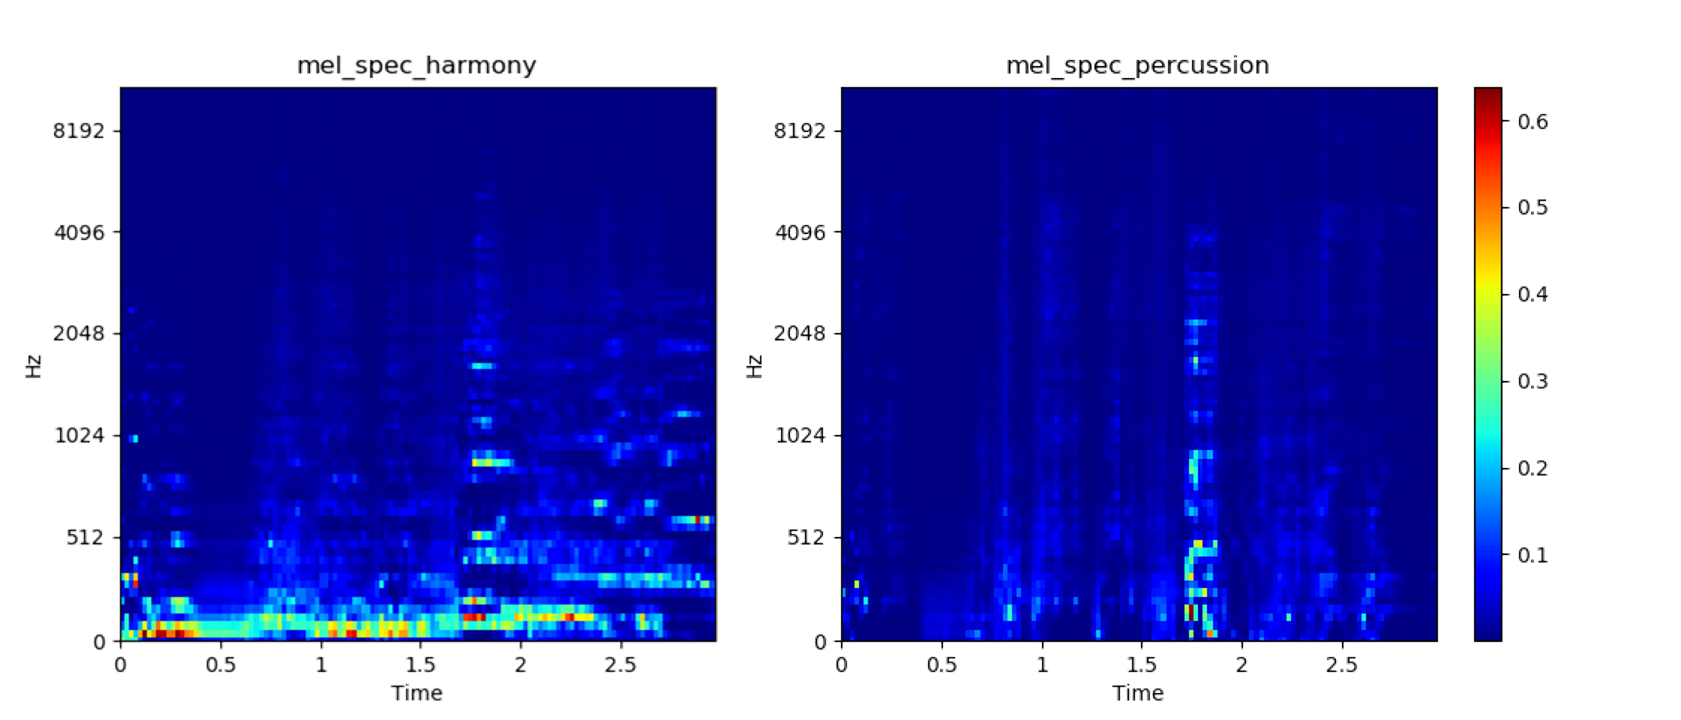
\includegraphics[scale=0.51]{./images/generate-model/gen-classical.png}
		\caption{Classicalと分類した生成スペクトログラム}
		\label{fig:generate-classical}
	\end{center}
\end{figure}
\begin{figure}[htbp]
	\begin{center}
		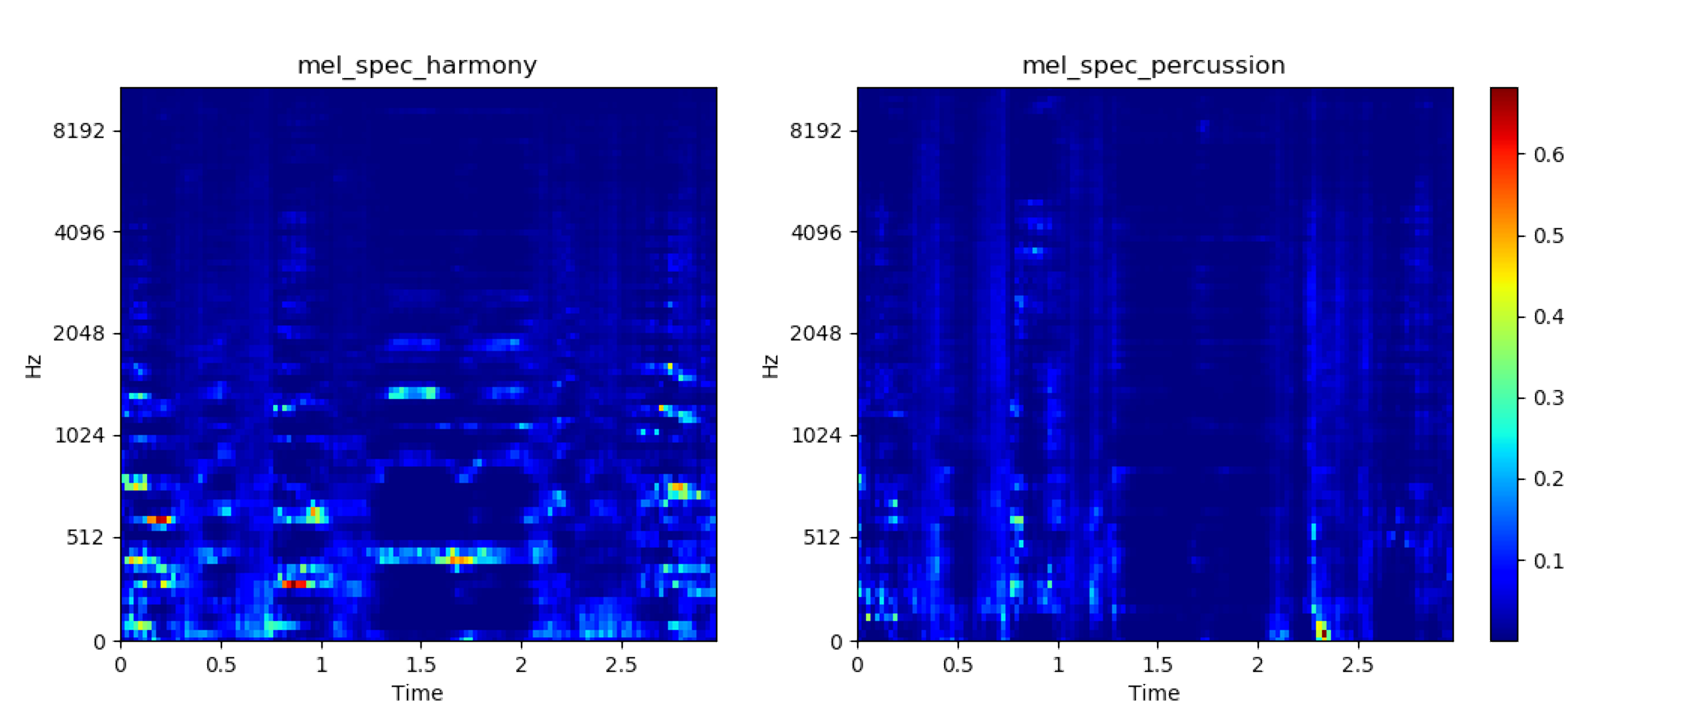
\includegraphics[scale=0.51]{./images/generate-model/gen-country.png}
		\caption{Countryと分類した生成スペクトログラム}
		\label{fig:generate-country}
	\end{center}
\end{figure}
\begin{figure}[htbp]
	\begin{center}
		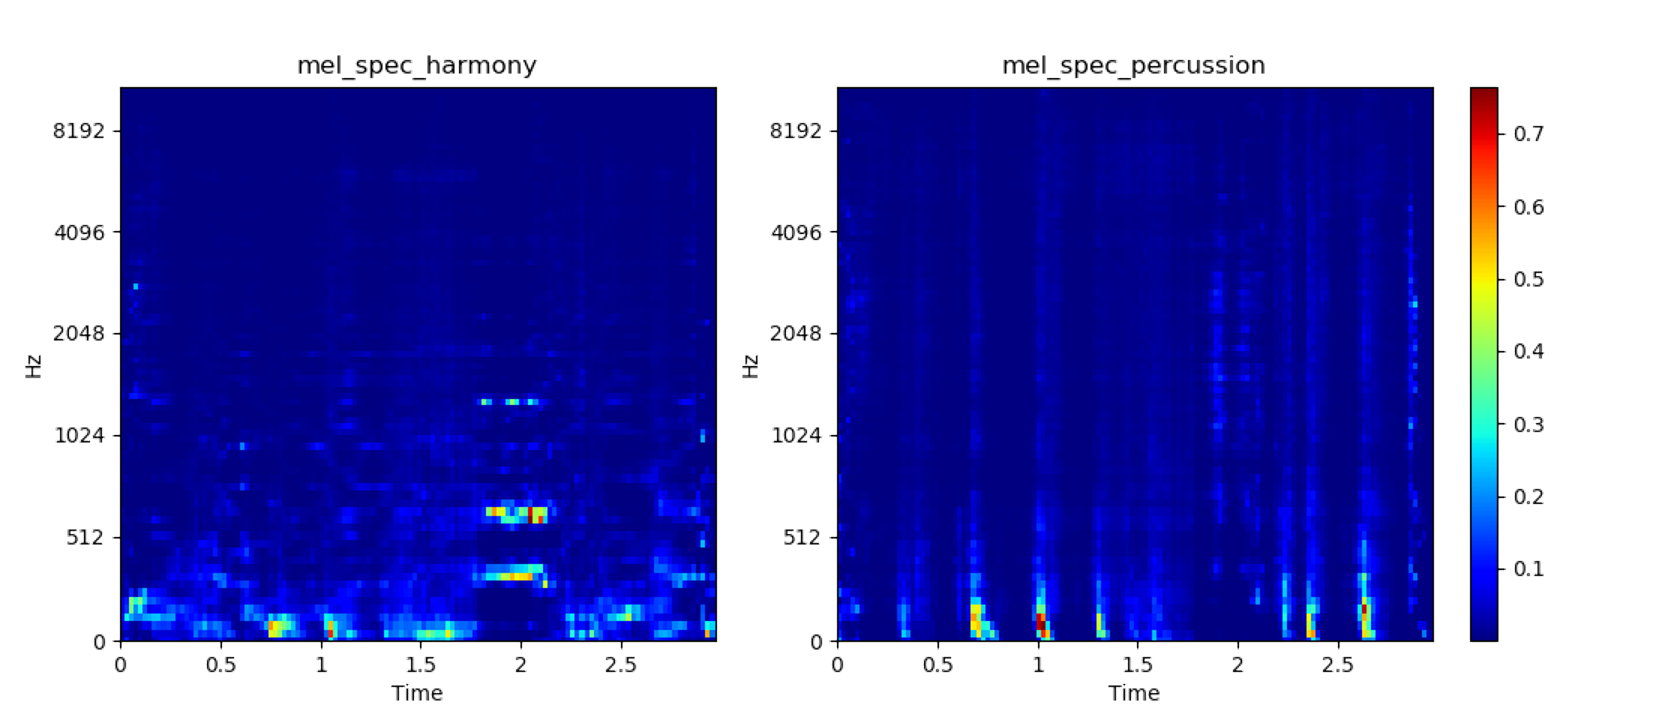
\includegraphics[scale=0.51]{./images/generate-model/gen-disco.png}
		\caption{Discoと分類した生成スペクトログラム}
		\label{fig:generate-disco}
	\end{center}
\end{figure}
\begin{figure}[htbp]
	\begin{center}
		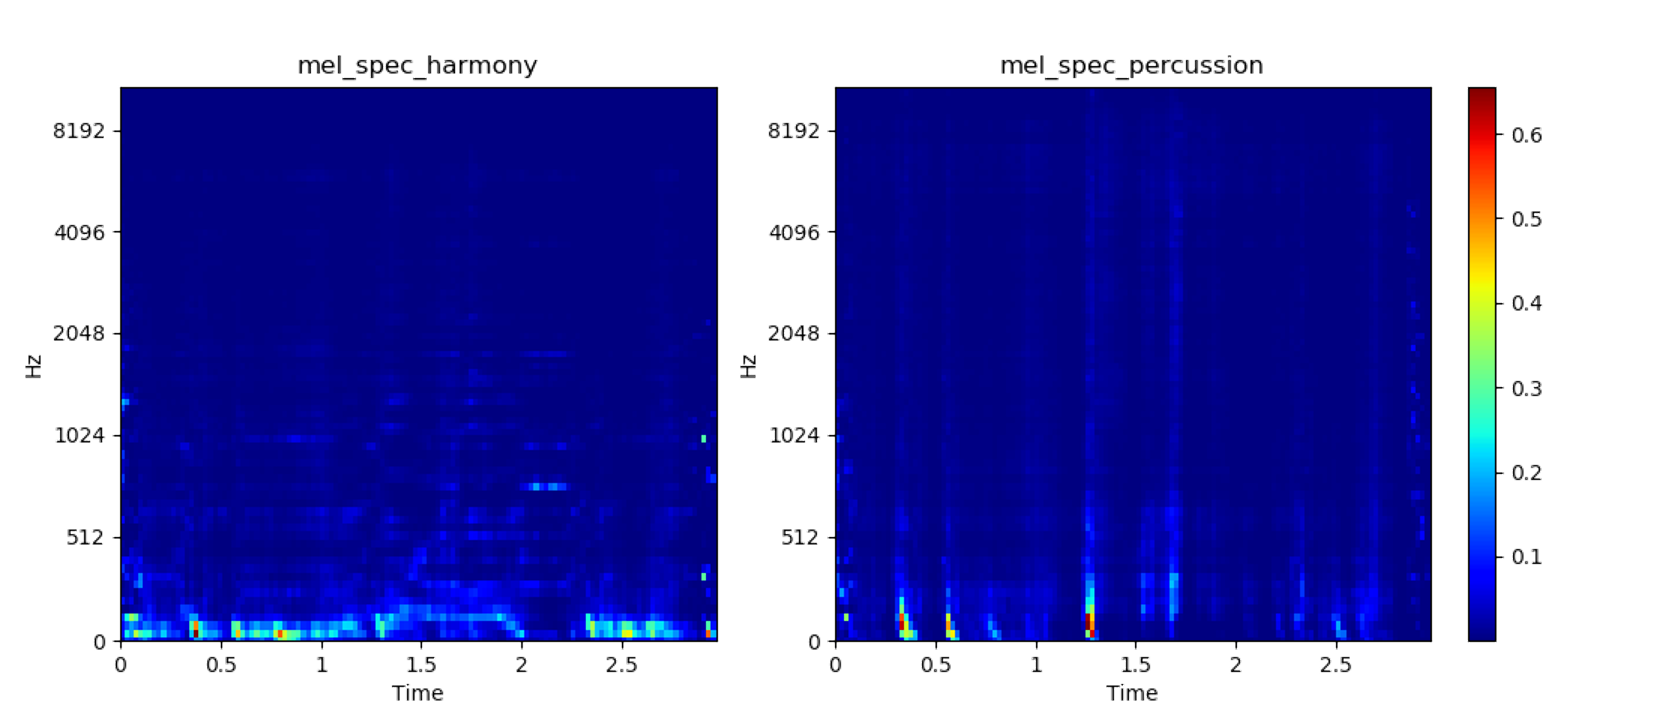
\includegraphics[scale=0.51]{./images/generate-model/gen-hiphop.png}
		\caption{Hiphopと分類した生成スペクトログラム}
		\label{fig:generate-hiphop}
	\end{center}
\end{figure}
\begin{figure}[htbp]
	\begin{center}
		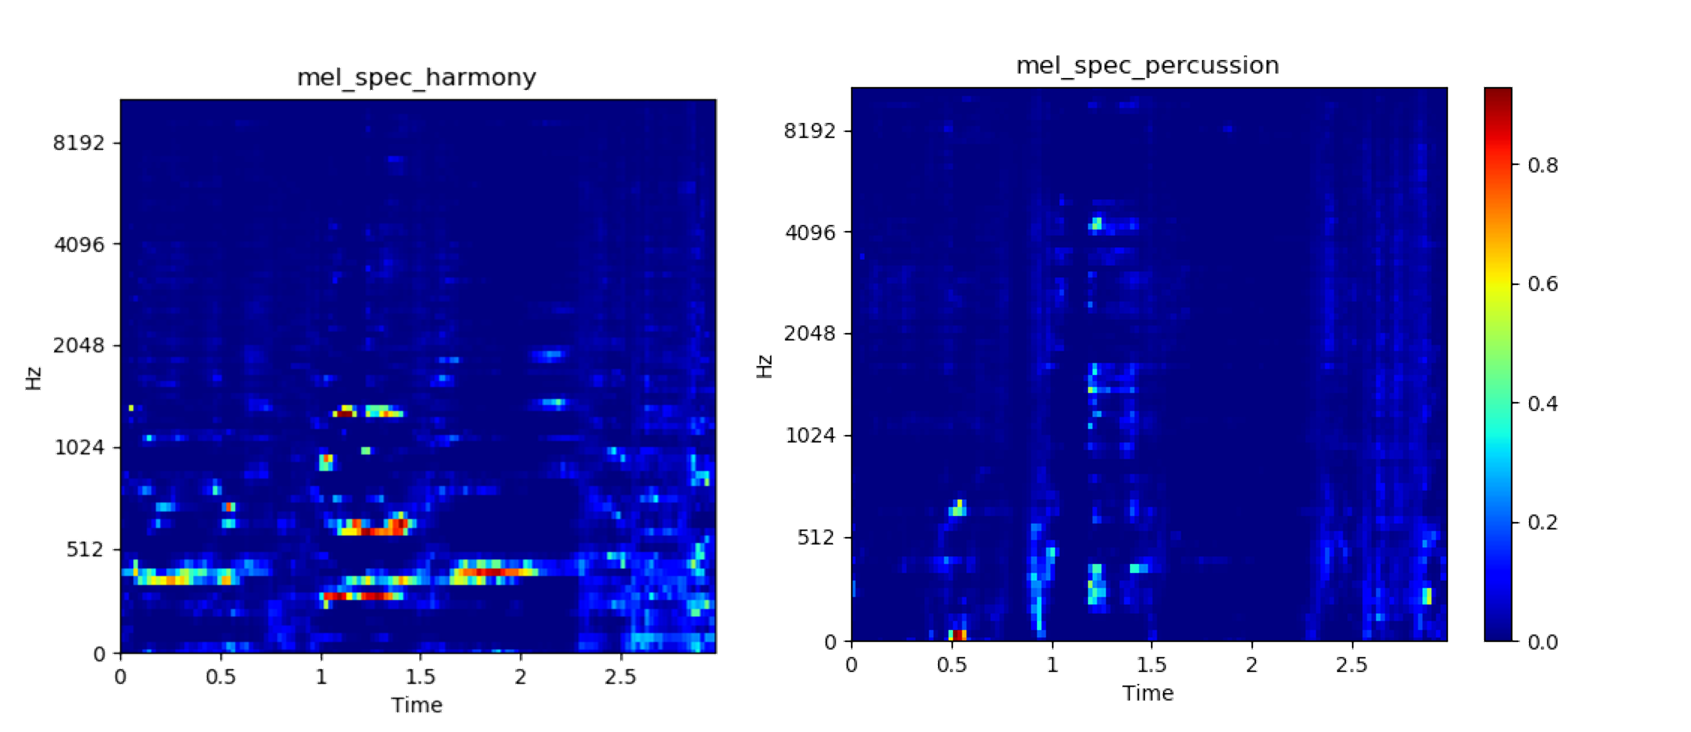
\includegraphics[scale=0.51]{./images/generate-model/gen-jazz.png}
		\caption{Jazzと分類した生成スペクトログラム}
		\label{fig:generate-jazz}
	\end{center}
\end{figure}
\begin{figure}[htbp]
	\begin{center}
		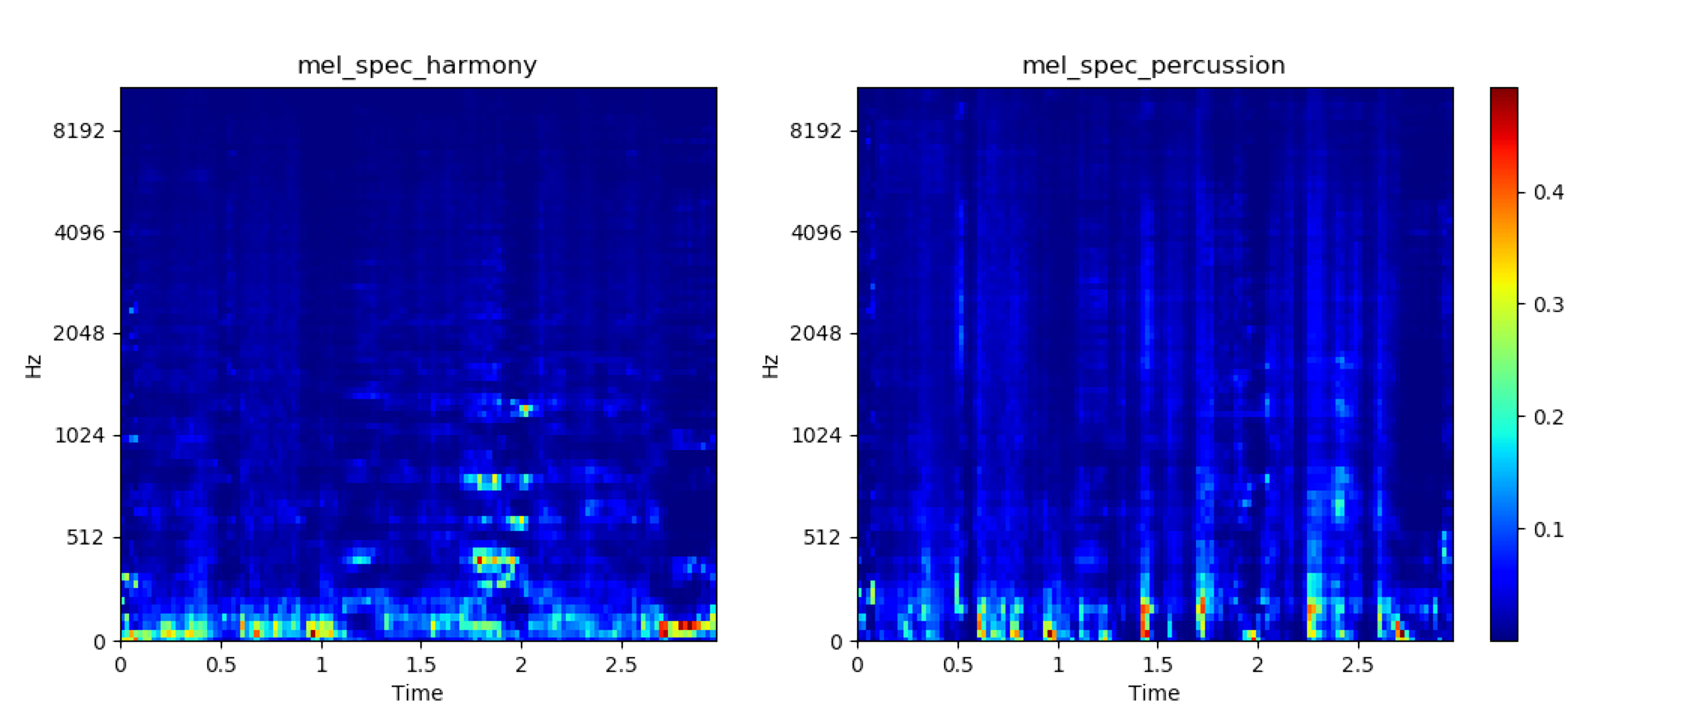
\includegraphics[scale=0.51]{./images/generate-model/gen-metal.png}
		\caption{Metalと分類した生成スペクトログラム}
		\label{fig:generate-metal}
	\end{center}
\end{figure}
\begin{figure}[htbp]
	\begin{center}
		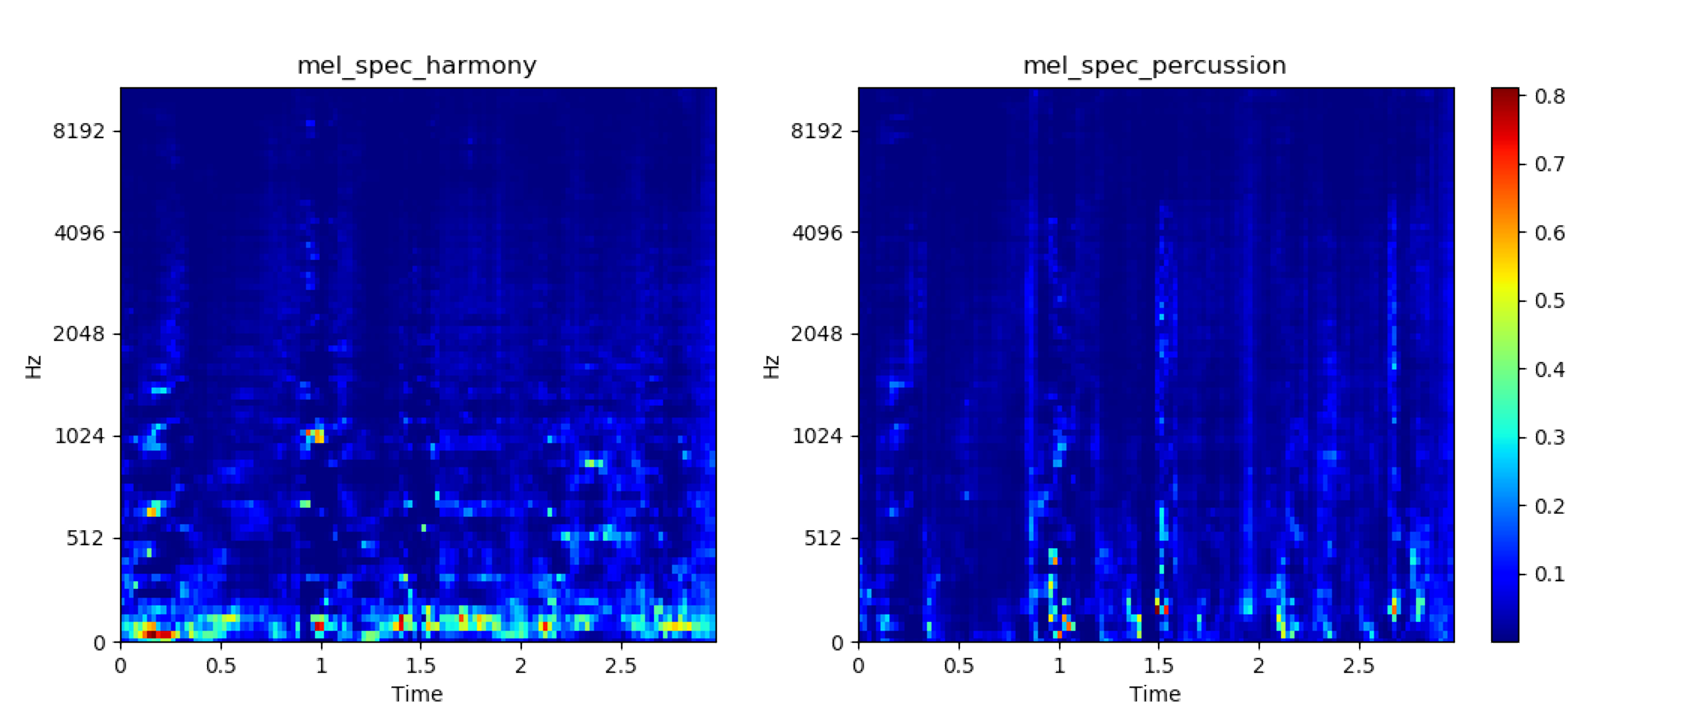
\includegraphics[scale=0.51]{./images/generate-model/gen-pop.png}
		\caption{Popと分類した生成スペクトログラム}
		\label{fig:generate-popl}
	\end{center}
\end{figure}
\begin{figure}[htbp]
	\begin{center}
		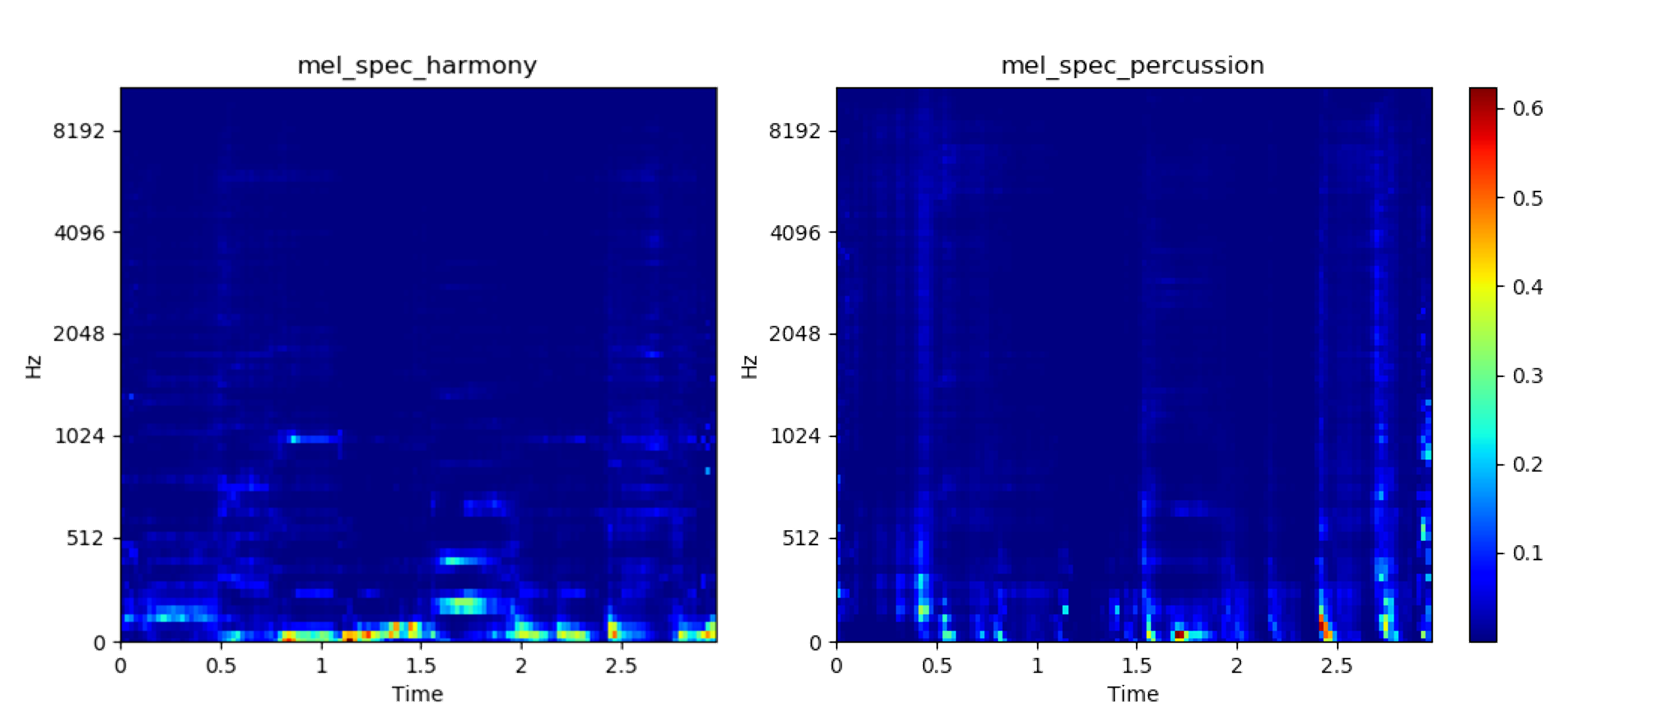
\includegraphics[scale=0.51]{./images/generate-model/gen-reggae.png}
		\caption{Reggaeと分類した生成スペクトログラム}
		\label{fig:generate-reggae}
	\end{center}
\end{figure}
\begin{figure}[htbp]
	\begin{center}
		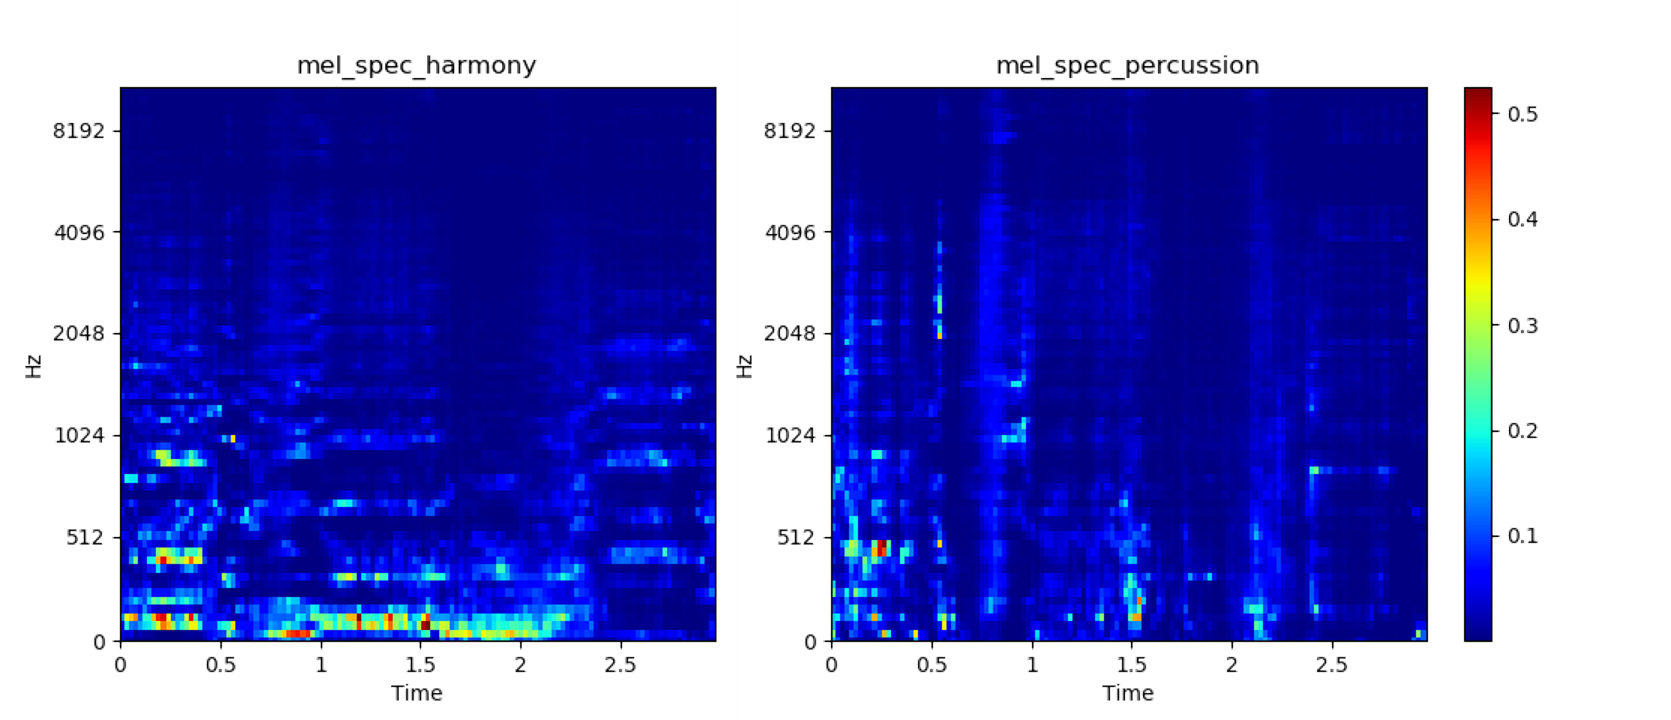
\includegraphics[scale=0.51]{./images/generate-model/gen-rock.png}
		\caption{Rockと分類した生成スペクトログラム}
		\label{fig:generate-rock}
	\end{center}
\end{figure}

\newpage
\figref{fig:generate-disco}と\figref{fig:generate-hiphop}より,DiscoとHip-hopにおいてはパーカッション成分で低周波に強めのビートが,特徴として表れやすいということが分かる.これはDiscoやHip-hopなどのダンス系の音楽は,バスドラムの音を他の音より強めに出す傾向があることと一致している.また,Metalにおいては,ハーモニー成分とパーカッション成分の両方のにおいて,強調される周波数が全帯域に広がりやすい傾向があることも読み取れる.これはギターの音を歪ませることにより多くの倍音が含まれるといった楽曲が多いためであると考えられる.

\subsection{生成スペクトログラムのジャンル確率分布}
生成されるスペクトログラムのジャンルの偏りを調べるために,一様乱数のシード値を変化させながら,バッチサイズ128のスペクトログラムを生成していく.これらを学習済みCNNで分類していき,最後にデータ総数で除算する.これにより生成されるスペクトログラムのジャンルの確率分布を求める.ジャンル毎の確率分布を\tabref{tab:prob-dist}に示す.
\tabref{tab:prob-dist}より,生成されるスペクトログラムのジャンルに偏りがあることが分かる.これは,Generatorがほぼ同一のデータしか出力しなくなるMode Collapseという現象に陥っているため,数ジャンルにだけ特化した生成モデルとなっている.それぞれのジャンルを均一に生成するためにはさらなる工夫が必要であると考えられる.
\begin{table}[htbp]
	\begin{center}
		\caption{ジャンル毎の生成確率分布}
		\scalebox{0.9}{{}
			\begin{tabular}{|c|c|c|} \hline
				ジャンル & 確率分布(\%)  \\ \hline
				Blues & 16.97 \\ \hline
				Country & 0.85 \\ \hline
				Classical & 17.56 \\ \hline
				Disco & 13.75 \\ \hline
				Hip-hop & 22.82 \\ \hline
				Jazz &18.13 \\ \hline
				Metal & 3.67\\ \hline
				Pop & 0.31 \\ \hline
				Reggae & 4.46 \\ \hline
				Rock & 4.79  \\ \hline
		\end{tabular}
		}
		\label{tab:prob-dist}
	\end{center}
\end{table}


\newpage
\section{2次元ジャンルマップの検証}
\figref{fig:featmap-trans}のように,2次元ジャンルマップ空間において,矢印の方向でジャンル境界を跨ぐように座標をずらしていき,そのときのジャンル出力確率の変化をグラフにしたものを\figref{fig:prob-trans}に示す.\figref{fig:prob-trans}は,横軸にマップの座標,縦軸にその時のジャンル毎の確率を表している.\\
次に$z_1=-0.57$で値を固定し,別の次元の従属ベクトル$z_6$を取り出し,$(z_0, z_6)$に関する2次元ジャンルマップ空間を作成したものを\figref{fig:featmap6}に示す.また$z_0=0.57$の軸で変化させたときのマップと出力確率の変化のグラフを\figref{fig:trans2}に示す.



\figref{fig:prob-trans}よりジャンル同士の出力確率が連続変化していることから,生成されるスペクトログラムはジャンルの特徴となるものが連続変化をしていると言える.また,確率の交差する点がジャンル境界となるため,その時に生成されるスペクトログラムがジャンルの中間データであると考えられる.\figref{fig:featmap-trans}と\figref{fig:prob-trans}から,マップの座標がジャンルの境界面に近づくにつれ,両者の確率がトレードオフに変化していき,境界上で確率がイーブンなる.すなわちマップはジャンル間に対する距離的な領域空間を表していると考えらえる.


一方,マップの座標$(z_0, z_1) = (0.57, -0.57)$付近のDiscoの領域において,Metalの確率が上がっていることについて考える.一見,マップにはMetalジャンルの領域は示されてはいないが,$z_1=-0.57$で値を固定した\figref{fig:featmap6}から,別次元のマップでMetalの領域が現れていることがわかる.さらに\figref{fig:trans2}からもわかるように,$(z_0, z_1) = (-0.57, 0.57)$で値を固定し$z6$を動かした時,DiscoとMetalの確率がトレードオフに変化していることからも,DiscoとMetalの距離空間的も近いことが示されている.

\newpage
\begin{figure}[htbp]
	\begin{center}
		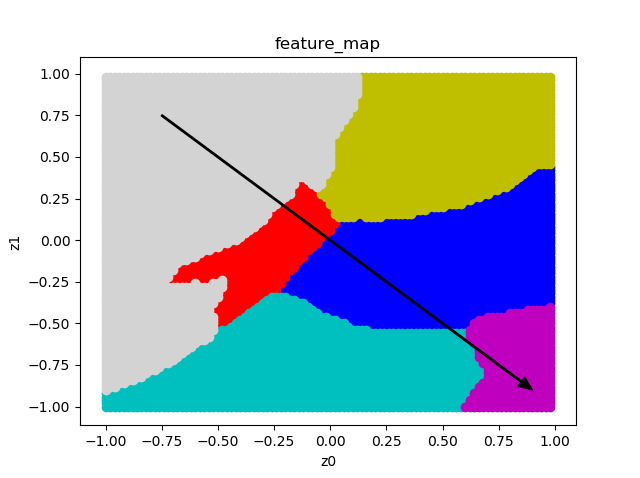
\includegraphics[scale=0.8]{./images/visualize/map_trans.png}
		\caption{ジャンルデータの変化}
		\label{fig:featmap-trans}
		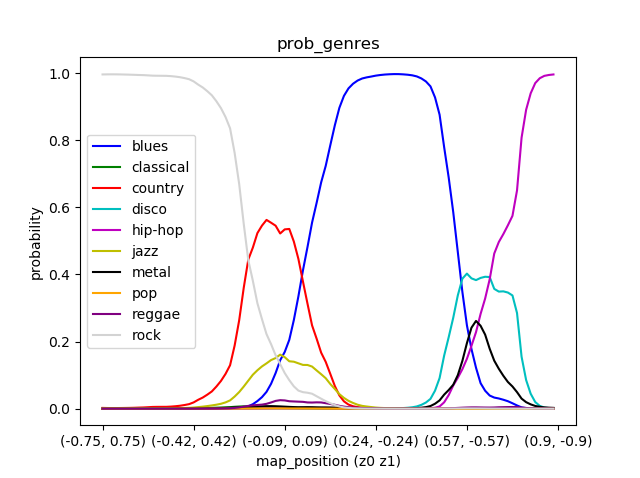
\includegraphics[scale=0.8]{./images/visualize/prob_trans.png}
		\caption{ジャンル毎の確率変化}
		\label{fig:prob-trans}
	\end{center}
\end{figure}

\begin{figure}[htbp]
	\begin{center}
		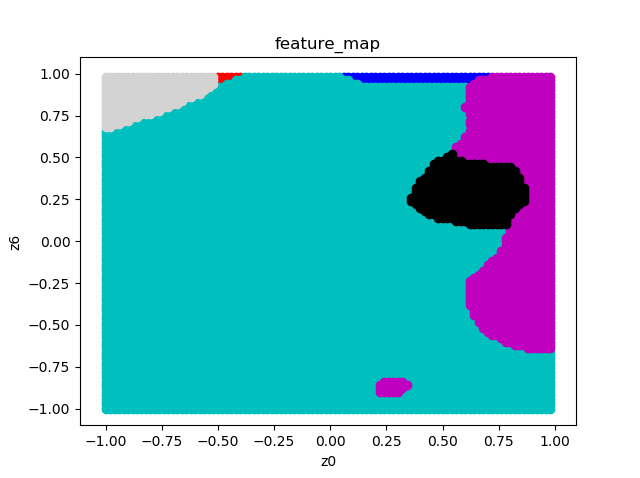
\includegraphics[scale=0.8]{./images/visualize/map6.png}
		\caption{$z_1=-0.57$における$(z_0, z_6)$のジャンルマップ}
		\label{fig:featmap6}
		\vspace{40pt}
		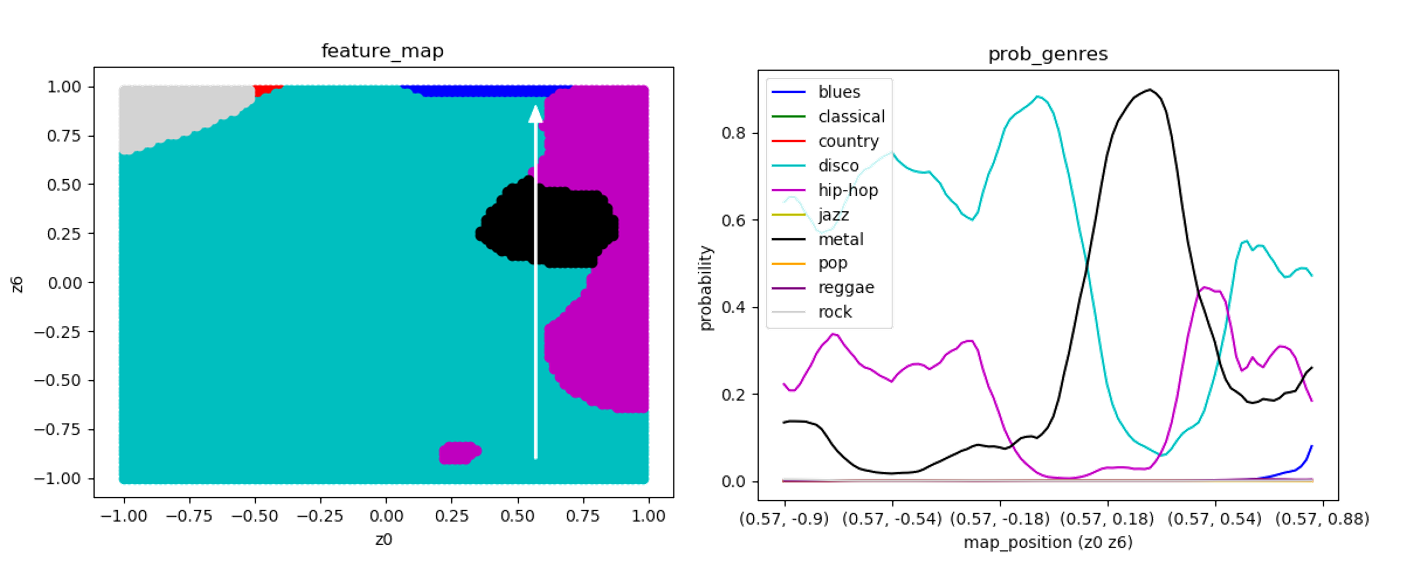
\includegraphics[scale=0.7]{./images/visualize/trans2.png}
		\caption{$z_0=0.57$におけるジャンル変化}
		\label{fig:trans2}
	\end{center}
\end{figure}
